\RequirePackage{plautopatch}
\documentclass[a4paper,10.5pt]{jsarticle}
%\documentclass[11pt]{ujarticle}

%%%%%%% スタイルファイル %%%%%%%%%%%%%%%%%%%%%%
\usepackage[T1]{fontenc}
\usepackage{lmodern}
\usepackage{amsmath,amssymb}
\usepackage{bm} % フォント設定のあとに読み込む

\usepackage[dvipdfmx]{graphicx}   % pdf 形式の図版取り込みのため
\usepackage{float}
\usepackage{array}
\usepackage{multicol}
\usepackage{ascmac}

\usepackage{eclbkbox}
\usepackage{indent}
\usepackage{report5s}

\usepackage{listings}
\usepackage{tcolorbox} % optional for colored boxes
\tcbuselibrary{listingsutf8} % for using listings inside tcolorbox (optional)


% \setlength\parindent{0zw}

\begin{document}

%-------------------------------------------------------------------------%
\thispagestyle{empty}
% !TEX root = main.tex

\renewcommand{\arraystretch}{0.8}

\begin{center}
  \begin{tabular}{|>{\centering\arraybackslash}p{12cm}|} \hline
    \\
    {\LARGE\textbf{制 御 工 学 実 験 報 告 書}} \\ 
    \\ \hline
  \end{tabular}
  
  \vspace*{0.55cm}
  
  \begin{tabular}{|p{15cm}|} \hline
    \\
    {\Large\textbf{ 実験テーマ:(4) PLCによるシーケンス制御}} \\
    \\ \hline
  \end{tabular}
  
  \vspace*{0.55cm}
  
  \begin{tabular}{|p{11cm}|} \hline
    \\
    {\large\textbf{   実験日  : 令和 6年11月29日}} \vspace*{0.25cm}           \\
    {\large\textbf{   \phantom{実験日  : 令和  年}12月06日}} \vspace*{0.25cm} \\
    {\large\textbf{   共同実験者:  3番 蘆田 修平}}                               \\ 
    {\large\textbf{          11番 岡本 陵平}}                               \\ 
    {\large\textbf{          19番 近藤 慧始}}                               \\ 
    {\large\textbf{          36番 宮武 駿}}                                 \\ 
    \\ \hline
  \end{tabular}
  
  \vspace*{0.25cm}
  
  \begin{tabular}{|p{11cm}|} \hline
    \\
    {\large\textbf{   提出日  : 令和  年  月  日}} \vspace*{0.25cm} \\
    {\large\textbf{   再提出日 : 令和  年  月  日}} \vspace*{0.25cm} \\
    {\large\textbf{   再々提出日: 令和  年  月  日}}                  \\
    \\ \hline
  \end{tabular}
  
  \vspace*{0.55cm}
  
  \begin{tabular}{|p{11cm}|} \hline
    \\
    {\large\textbf{   5 S    28番}} \vspace*{0.25cm} \\
    {\large\textbf{   氏名   :野口 史遠 }}            \\
    \\ \hline
  \end{tabular}
  
  \vspace*{0.55cm}
  
  \begin{itembox}[r]{\textbf{コメント}}
    \hspace*{12.5cm} \\
    \hspace*{12.5cm} \\
    \hspace*{12.5cm} \\
    \hspace*{12.5cm} \\
    \hspace*{12.5cm} \\
    \hspace*{12.5cm} \\
    \hspace*{12.5cm} \\
    \hspace*{12.5cm} \\
    \hspace*{12.5cm} \\
    \hspace*{12.5cm} \\
    \hspace*{12.5cm} \\
    \hspace*{12.5cm} \\
  \end{itembox}
\end{center}
\renewcommand{\arraystretch}{1}

\newpage

% \pagenumbering{roman}
% \setcounter{page}{1}

% \tableofcontents    %% 目次 
% \newpage

\pagenumbering{arabic}
\setcounter{page}{1}
%-------------------------------------------------------------------------%
%%%%%%%%%%%%%%%%%%%%%%%%%%%%%%%%%%%%%%%%%%%%%%%%%%%%%%%%%%%%%%%%%%%%%%%%%%%%%
%%%%%% 本文 %%%%%%%%%%%%%%%%%%%%%%%%%%%%%%%%%%%%%%%%%%%%%%%%%%%%%%%%%%%%%%%
%%%%%%%%%%%%%%%%%%%%%%%%%%%%%%%%%%%%%%%%%%%%%%%%%%%%%%%%%%%%%%%%%%%%%%%%%%%%%

%\rule{1\textwidth}{1mm}\vspace*{0.15cm}
\begin{center}
  {\huge\textbf{(3) 倒立振子のパラメータ同定と安定化}}
\end{center}
%\rule{1\textwidth}{1mm}
\vspace*{1cm}


%% !TEX root = main.tex

\section{実験目的}

産業用ロボットの多くは,複数のリンクと回転関節から構成されるシリアルリンク型である.
本実験では,6自由度垂直多関節型のマニピュレータを用いて,
ティーチングと呼ばれる産業用ロボットのプログラムを作成する方法を学ぶ.
また,マニピュレータの制御で用いられる運動学の基礎知識を習得する.
さらに,カメラを用いた物体検知と3次元位置計測を通じて,ロボットビジョンの基礎技術を学ぶ.


\section{多自由度マニピュレータ}

\subsection{ティーチング}
マニピュレータ(産業用ロボット)の制御は,運動学や軌道決定を計算し,
モータを制御するなどのマニピュレータの動きを含めた制御に分けて考える必要がある.
前者については,4年後期の講義「ロボティクスII」にて基礎知識を学ぶ.
後者のマニピュレータへの動作入力方法には,ティーチングとよばれる表示方法が用いられている.

ティーチングは,ダイレクトティーチング,オンラインティーチング,オフラインティーチングに分類される.
ダイレクトティーチングはマニピュレータ本体に直接(ダイレクト)
に触れながらマニピュレータの動作を記録し,記録した動作をプレイバック(再現)する.
オンラインティーチングはティーチングペンダントと呼ばれるインターフェイスを使用して,
マニピュレータを手動操作し,動作を記録,プレイバックさせる.
オフラインティーチングは,コンピュータ上でシミュレータを操作し,
動作を記録する.そして,実際のマニピュレータにデータを送信し,
プレイバックさせる方法である.

\subsection{システム構成}
本実験で用いる多自由度マニピュレータは,xArm 6(UFACTORY製)である.
6個の回転関節を有するため,自由度は3次元空間の位置姿勢を任意に決めることができる6自由度である.
各関節はサーボモータによって駆動され,関節角度はアブソリュート型エンコーダによって取得される.

本実験システムは,マニピュレータ,空圧駆動型ロボットグリッパおよび制御PC,
ノートPCから構成される.図2.1にマニピュレータのシステム構成を示す.
制御PCはLinuxと呼ばれるOSが搭載されており,制御周期10msでマニピュレータを制御している.
制御PC内では,マニピュレータの運動学,姿勢,軌道の計算,モータの制御などが行われており,
マニピュレータの動きを統合的にコントロールしている.
ノートPCは専用の制御ソフトウェアを用いることで,マニピュレータの手動操作,
状態の確認やティーチング,各種設定を行うことができる.
つまり,ティーチングペンダントと同等の操作ができる.
また,Pythonを用いることで,ロボットビジョンやAIを活用したマニピュレータへの動作指示の送信や,
マニピュレータの状態を受信することも可能である.

\begin{figure}[h]
  \centering
  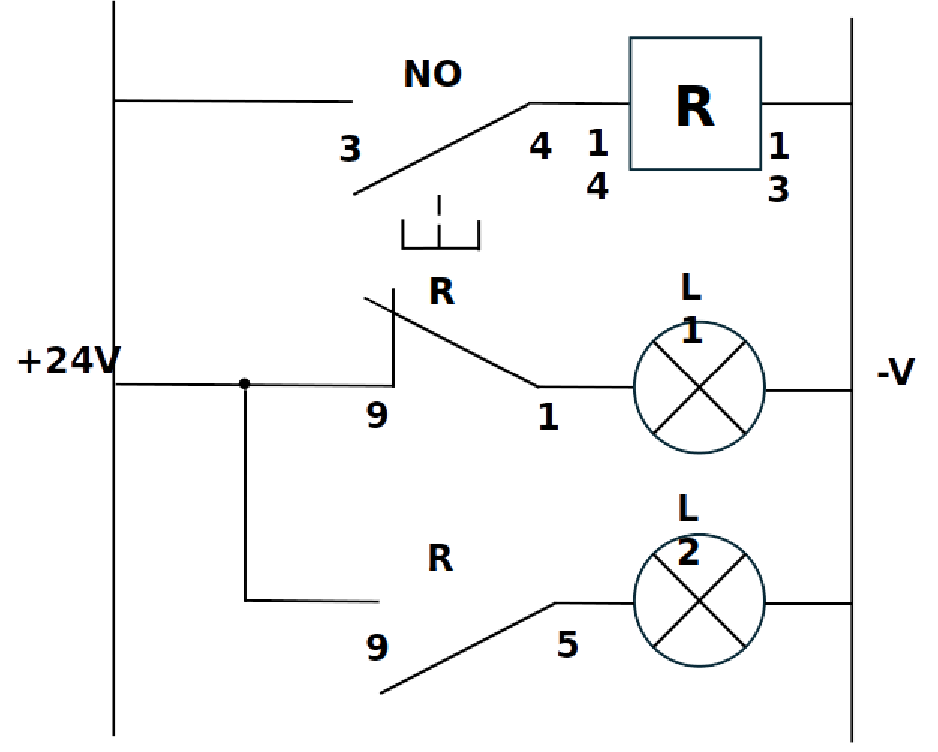
\includegraphics[scale=1]{sozai/1.pdf}
  \caption{システム構成}
\end{figure}


\subsection{マニピュレータの運動学}
各関節角度を入力として,手先の位置姿勢を求める問題を順運動学という.
一方で,手先の位置姿勢を入力として各関節角度を求める問題を逆運動学という.
本実験では,マニピュレータの第4~第6関節を固定し,
3自由度マニピュレータとして運動学を考える.
これは,マニピュレータを簡単な構造として,運動学を幾何学計算するためである.

\subsubsection{順運動学}
グローバル座標系$\Sigma_0$の原点から$z_0$軸方向に$l_1$平行移動した
座標系$\Sigma$からみた手先位置を計算する.幾何学的に考える場合,
まず$x'z'$平面で考える.三角関数を用いると,手先位置$[x' \ z']^T$は,

\begin{align}
  x' & = l_2 \cos (\varphi_1 - \theta_2) - l_3 \cos \{ (\varphi_1 - \theta_2) + (\varphi_2 - \theta_3) \} \tag{2.1} \\
  z  & = l_2 \sin (\varphi_1 - \theta_2) - l_3 \sin \{ (\varphi_1 - \theta_2) + (\varphi_2 - \theta_3) \} 
\end{align}

となる.次に,座標系$\Sigma$の原点から手先位置を$xy$平面に射影すると,
式(2.1)より大きさ$|x'|$を用いて,

\begin{align}
  x & = |x'| \cos \theta_1 \tag{2.2} \\
  y & = |x'| \sin \theta_1 
\end{align}

と計算することができる.また,グローバル座標系$\Sigma_0$からみた手先位置は,
式(2.1),式(2.2)を用いて,

\begin{align}
  \begin{bmatrix}
    x \\
    y \\
    z
  \end{bmatrix}
  = 
  \begin{bmatrix}
    x \\
    y \\
    z + l_1
  \end{bmatrix} \tag{2.3}
\end{align}

となる.

\subsubsection{逆運動学}
逆運動学について説明する.グローバル座標系からみた手先位置
$\begin{bmatrix} x_0 \ y_0 \ z_0 \end{bmatrix}^T$が既知の場合,

\begin{align}
  \begin{bmatrix} x \\ y \\ z \end{bmatrix} = \begin{bmatrix} x_0 \\ y_0 \\ z_0 - l_1 \end{bmatrix} \tag{2.4}
\end{align}

と座標系$\Sigma$からみた手先位置を求めることができる.
つまり,手先位置$[x \ y \ z]^T$が既知となった.
次に,座標系$\Sigma$の$xy$平面を考えると,関節角度$\theta_1$は,

\begin{align}
  \theta_1 = \tan^{-1} \frac{y}{x} \tag{2.5}
\end{align}

と$x, y$を用いて計算できる.なお,$x^2 + y^2 = 0$のときは,
$\theta_1$は一意に決まらず,任意の値になる.ここで,アークタンジェントは,
プログラミング言語において$\text{atan}$と$\text{atan2}$の2種類存在する.
今回は,戻り値の範囲が広い$\text{atan2}$を使用する.

\begin{align}
  \theta_1 = \text{atan2}(y, x) \tag{2.6}
\end{align}

以下,アークタンジェントは$\text{atan2}$で表記する.

次に関節角度$\theta_3$を余弦定理から求める.
先に計算に必要な$x'$について求める.
$xy$平面の原点から手先位置を射影した点までの長さは

\begin{align}
  |x'| = \sqrt{x^2 + y^2} \tag{2.7}
\end{align}

と$x, y$を用いて計算できる.絶対値を外すと,

\begin{align}
  x' = \pm \sqrt{x^2 + y^2} \tag{2.8}
\end{align}

である.この値を用いて余弦定理を適用する.
余弦定理は,三角形$ABC$に対し,辺$AB, AC$のなす角を$\theta$とすると,

\begin{align}
  BC^2 = AB^2 + AC^2 - 2 AB \cdot AC \cos \theta \tag{2.9}
\end{align}

という関係式が成立する定理である.$x'z'$平面の三角形に注目すると,
余弦定理を適用して

\begin{align}
  \cos(\varphi_2 - \theta_3) = \frac{l_2^2 + l_3^2 - x'^2 - z^2}{2 l_2 l_3} \tag{2.10}
\end{align}

が成立する.

また,$\sin^2 \theta + \cos^2 \theta = 1$の関係から,

\begin{align}
  \sin(\varphi_2 - \theta_3) = \pm \sqrt{1 - \cos^2 (\varphi_2 - \theta_3)} \tag{2.11}
\end{align}

となるため,式(2.6)と同様に$\text{atan2}$を用いると,

\begin{align}
  \theta_3 = \varphi_2 - \text{atan2} \{ \sin(\varphi_2 - \theta_3), \cos(\varphi_2 - \theta_3) \} \tag{2.12}
\end{align}

となる.

最後に,関節角度$\theta_2$を求める.
上記で求めた関節角度$\theta_3$の値が既知になったと考えると,
順運動学で求めた式(2.1)を$\cos(\varphi_2 - \theta_2), \sin(\varphi_2 - \theta_2)$の連立方程式として考えることができる.連立方程式を解くと,

\begin{align}
  \cos(\varphi_1 - \theta_2) = \frac{K_c x' + K_s z}{K_c^2 + K_s^2}, \quad \sin(\varphi_1 - \theta_2) = \frac{K_s x' + K_c z}{K_c^2 + K_s^2} \tag{2.13}
\end{align}

と解を導出できる.$\text{atan2}$を用いると,

\begin{align}
  \theta_2 = \varphi_1 - \text{atan2} \{ \sin(\varphi_1 - \theta_2), \cos(\varphi_1 - \theta_2) \} \tag{2.14}
\end{align}

となる.
なお,本実験では逆運動学の式中に正負が混在している場合はすべて正の場合で考えるものとする.



\subsection{マニピュレータの姿勢表現}
マニピュレータの手先姿勢は2つの座標系$\Sigma_0$と$\Sigma_e$を用いて表現することができる.
グローバル座標系$\Sigma_0$はマニピュレータのベースに固定された静止座標系であり,
手先座標系$\Sigma_e$はロボットアームの手先に固定された座標系である.

手先の姿勢を表現する際は,座標系$\Sigma_0$からみた座標系$\Sigma_e$の各軸($e_x, e_y, e_z$)
の単位ベクトル$0\mathbf{e}_x, 0\mathbf{e}_y, 0\mathbf{e}_z$を用いる.
単位ベクトルとは,大きさ(長さ)が1のベクトルである.
つまり,$0\mathbf{e}_x, 0\mathbf{e}_y, 0\mathbf{e}_z$はそれぞれ座標系$\Sigma_e$の軸
($e_x, e_y, e_z$)方向を向く大きさ1のベクトルを意味している.この3つのベクトルをまとめて,
$3 \times 3$の行列で表記されたものを回転行列と呼ぶ.

\begin{align}
  ^0\mathbf{x}_{P} = \begin{bmatrix} r_{11} \\ r_{21} \\ r_{31} \end{bmatrix}, \quad ^0\mathbf{e}_y = \begin{bmatrix} r_{12} \\ r_{22} \\ r_{32} \end{bmatrix}, \quad ^0\mathbf{e}_z = \begin{bmatrix} r_{13} \\ r_{23} \\ r_{33} \end{bmatrix}
\end{align}

\begin{align}
  ^0\mathbf{R} = \begin{bmatrix} ^0\mathbf{e}_x & ^0\mathbf{e}_y & ^0\mathbf{e}_z \end{bmatrix} = \begin{bmatrix} r_{11} & r_{12} & r_{13} \\ r_{21} & r_{22} & r_{23} \\ r_{31} & r_{32} & r_{33} \end{bmatrix} \tag{2.16}
\end{align}

回転行列よりもわかりやすく姿勢を表現する方法として,固定角やオイラー角と呼ばれる方法がある.
本実験ではxArm 6に採用されている固定角を用いる.
固定角は,座標系$\Sigma_0$を基準に次の3つの連続する回転で表現する.
(1)の軸まわりの「roll」回転,(2)の軸まわりの「pitch」回転,
(3)の軸まわりの「yaw」回転である.3つの連続回転により,
任意の姿勢を表現することができる.回転行列では3つの角のパラメータが必要であったが,
固定角では$\psi, \theta, \phi$の3つのパラメータで姿勢を表現することができる.
ここで,xArm 6ではなくロボットアーム上の$\psi, \theta, \phi$をピッチ角$P, \phi$をヨー角$Y, R$
と呼称している.

また,固定角の$\psi, \theta, \phi$が既知のとき,回転行列$\mathbf{R}$は,

\begin{align}
  ^0\mathbf{R} = R_z R_y R_x = 
  \begin{bmatrix} 
    \cos \psi \cos \theta & \cos \psi \sin \theta \sin \phi - \sin \psi \cos \phi & \cos \psi \sin \theta \cos \phi + \sin \psi \sin \phi \\ 
    \sin \psi \cos \theta & \sin \psi \sin \theta \sin \phi + \cos \psi \cos \phi & \sin \psi \sin \theta \cos \phi - \cos \psi \sin \phi \\ 
    - \sin \theta         & \cos \theta \sin \phi                                 & \cos \theta \cos \phi 
  \end{bmatrix} \tag{2.17}
\end{align}

となり,$\psi, \theta, \phi$を軸まわりにそれぞれ単位回転した際の回転行列$\mathbf{R}$で
計算することができる.また,回転行列の各要素が既知のときは,

\begin{align}
  \theta = \text{atan2} \left( -r_{31}, \pm \sqrt{r_{11}^2 + r_{21}^2} \right) \tag{2.18}
\end{align}

\begin{align}
  \psi = 
  \begin{cases}
    \text{atan2}(r_{21}, r_{11})   & \text{if } \cos \theta > 0, \\
    \text{atan2}(-r_{21}, -r_{11}) & \text{if } \cos \theta < 0
  \end{cases} \tag{2.19}
\end{align}

\begin{align}
  \phi = 
  \begin{cases}
    \text{atan2}(r_{32}, r_{33})   & \text{if } \cos \theta > 0, \\
    \text{atan2}(-r_{32}, -r_{33}) & \text{if } \cos \theta < 0
  \end{cases} \tag{2.20}
\end{align}

と計算できる.この計算は,式(2.16)と式(2.17)の各要素を比較し,方程式を立式することで求めることができる.
式(2.16)の値を反映して,それぞれの求め方は以下の通りである.


- ピッチ角$\theta$:(1.1)要素を乗じて和を取る.また,(3.1)要素を用いて,$\text{atan2}$を用いる.


- ヨー角$\psi$:(1.1)要素および(2.1)要素を比較して,$\text{atan2}$を用いる.


- ロール角$\phi$:(3.2)要素および(3.3)要素を比較して,$\text{atan2}$を用いる.


\section{ロボットビジョン}

\subsection{概要}
マニピュレータは,カメラによる画像処理を組み合わせることで,
用途の幅を広げることができる.
ステレオカメラ(RGB-Dカメラ)を取り付けることで,対象物体の3次元位置情報を得ることができる.
そして,その位置情報を利用することで,把持対象の検出や手先位置の微調整が可能となる.
この一連の作業をリアルタイムで実行できるとすれば,カメラが介在したフィードバックシステム
(ビジュアルフィードバックシステムと呼ばれる)が完成する.

本実験では画像処理による対象物体の3次元位置計測を行う.
そして,位置情報からマニピュレータの手先位置を決定し,オンラインティーチングによる動作の入力を行う.

\subsection{画像処理}
本実験では,次の手順で画像処理を行い,3次元位置を計測する.

\begin{enumerate}
  \item[(1)] \textbf{画像の取得}:カメラから取得される画像は,カラー画像であり,赤色成分(R),緑色成分(G),青色成分(B)から構成されている.それぞれの成分は,0から255の256諧調の値を持つため,1画素(pixel)は3バイトである.色はRGB色空間とHSV色空間と呼ばれる2つの色の表現方法がある.本実験ではHSV色空間で画像を処理する.
    
  \item[(2)] \textbf{空間フィルタリング}:画像には外乱光などの影響により色の明るさやコントラストなどが変化する.その変化を低減するために,画像フィルタを通す.本実験では,空間フィルタリングと呼ばれる「平均化フィルタ」,「ガウシアンフィルタ」,「メディアンフィルタ」,「双方向フィルタ」をそれぞれ用いる.
    
  \item[(3)] \textbf{2値化処理}:HSV色空間から特定の色を検出し,白黒画像を生成する.これは2値化と呼ばれる処理を行う.2値化は任意の値(しきい値)を定め,それを基準として,各ピクセルを白または黒に割り当てる.この操作によって,抽出したい物体をそれ以外と区別する.実際,しきい値の決定方法には,Pタイル法,判別分析法,傾分といった手法など多岐にわたるが,ここではヒストグラムを参考に試行錯誤して決定するものとする.この2値化処理によって対象物体が特定できる画像が得られる.
    
  \item[(4)] \textbf{特徴パラメータの抽出}:対象物体の特徴となる値は,面積,周囲長,重心位置,形状などが考えられる.本実験では,画像全体を1つの物体と仮定し,2値化された白部分の面積と重心位置を求める.この重心位置を3次元位置計測に利用する.
    
  \item[(5)] \textbf{ステレオ法による3次元位置の計測}:2台のカメラ画像それぞれにある(4)で取得した画像上の物体の重心位置から三角測量の原理を用いると,3次元位置を計測できる.また,本実験で使用するステレオカメラ(Realsense D435f)にはプロジェクタによるパターンが照射されており,そのパターンを2台のカメラが検出することでカメラ画像同士のマッチングを行っている.
\end{enumerate}

\subsection{座標変換}
カメラから取得された画像はマニピュレータのグローバル座標系とは異なる視点を持っている.
そこで,カメラに固定された座標系からみた対象物体の位置を,
グローバル座標系に変換して考える必要がある.
本実験では,マニピュレータの手先にカメラが固定されているため,
カメラに固定された座標系は手先座標系$\Sigma_e$と等しいものとして考える.

座標を変換するには,グローバル座標系$\Sigma_0$の原点から手先座標系$\Sigma_e$の原点までの
位置ベクトル$^0\mathbf{p}_{0,e}$と,手先の姿勢を表す回転行列$^0\mathbf{R}$を用いて,

\begin{align}
  ^0\mathbf{x}_{P} = ^0\mathbf{p}_{0,e} + ^0\mathbf{R} \mathbf{x}_{P} \tag{3.1}
\end{align}

と計算する.
ここで,$^0\mathbf{x}_{P}$はグローバル座標系からみた対象物体,$\mathbf{x}_{P}$は
手先座標系からみた対象物体の3次元位置座標を示している.
本実験では,$^0\mathbf{p}_{0,e}$がマニピュレータの手先位置,
$\mathbf{x}_{P}$が求めたい対象物体の3次元位置,$^0\mathbf{x}_{P}$がカメラから
取得した対象物体の3次元位置,$^0\mathbf{R}$がマニピュレータの手先姿勢となる.
ただし,マニピュレータの制御用ソフトウェアでは,XYZオイラー角で姿勢が表現されるため,
$^0\mathbf{R}$に変換する必要がある.


\section{実験1-1:ティーチング実験}

\subsection{実験概要}
本実験では,図4.1中に示された番号の位置で試験管を模したホワイトボードマーカーを
抜き差しするマニピュレータの動作をダイレクトティーチングおよびオンラインティーチングを
用いて制御PCに入力する.P1~P3の位置には部品が配置されており,
その部品をそれぞれS1~S3に運搬する.また,運搬の途中で試験管を3回振る動作も行う.

\begin{figure}[h]
  \centering
  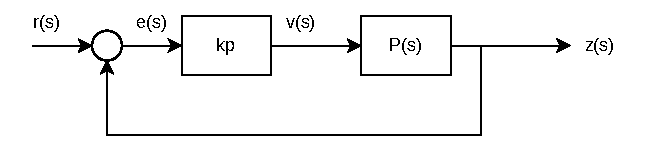
\includegraphics[scale=0.6]{sozai/2.pdf}
  \caption{実験環境(実験1)}
\end{figure}

\subsection{ダイレクトティーチング実験}

\subsubsection{実験手順}
実験は次の手順で行う.

\begin{enumerate}
  \item[(1)] 空圧駆動型ロボットグリッパの電磁弁を操作し,ホワイトボードマーカーを把持させる.
  \item[(2)] マニピュレータを初期位置姿勢付近に移動させる.
  \item[(3)] マニピュレータ制御用ソフトウェアからダイレクトティーチングを実行する.
  \item[(4)] 初期姿勢からS1上部に移動する.
  \item[(5)] S1とP1の中間地点で,ホワイトボードマーカーを3回振る.
  \item[(6)] P1の挿入口にホワイトボードマーカーを指す.
  \item[(7)] マニピュレータを初期位置姿勢付近に戻し,ダイレクトティーチングを終了する.
  \item[(8)] 記録した動作をプレイバックする.プレイバックの様子は動画撮影する.
  \item[(9)] P2とS2,P3とS3の組み合わせでもダイレクトティーチングを実行する.ただし,実行する人を交代させる(全員1度は実行すること(重複してもよい)).実行中の様子を適宜写真,動画撮影し,ティーチングに苦労している点および改善すべき点などを観察する.撮影した写真は考察などに利用する.利用する場合は図として載せること.
\end{enumerate}

\subsubsection{実験結果}
ダイレクトティーチングの実行結果について説明する.
図4.3にダイレクトティーチングのプレイバックの様子を示す.

\subsubsection{考察}
次に,実行結果について考察する.

\subsection{オンラインティーチング実験}

\subsubsection{実験手順}
マニピュレータ制御用ソフトウェアを用いて,オンラインティーチングを行う.
オンラインティーチングはビジュアルプログラミングモードを用いて行う.実験は次の手順で行う.

\begin{enumerate}
  \item[(1)] マニピュレータを初期位置姿勢に移動させる.
  \item[(2)] マニピュレータ制御用ソフトウェアからオンラインティーチングを実行する.
  \item[(3)] 初期姿勢からS1に移動し,ホワイトボードマーカーを把持する動作を行う.その後,ホワイトボードマーカーをS1から抜く.
  \item[(4)] S1とP1の中間地点で,ホワイトボードマーカーを3回振る.なお,マーカーを振る動作のティーチングは最初の1名が行い,その後はティーチングのデータを複製して使用してよい.
  \item[(5)] P1の挿入口にホワイトボードマーカーを指す.
  \item[(6)] マニピュレータを初期位置姿勢に戻す.
  \item[(7)] P2とS2,P3とS3の組み合わせでも同様にティーチングを行う.ただし,実行する人を交代すること.そして,全員1度は実行すること.人数が4人以上いる場合は,挿入口をP1,P2のホワイトボードマーカーをS1,S2にそれぞれ異なる動作にする.実行中の様子を適宜撮影し,ティーチングに苦労している点などを観察する.撮影した写真は考察などに利用する.利用する場合は図として載せること.
  \item[(8)] オンラインティーチングを終了する.
  \item[(9)] 記録した動作をプレイバックする.プレイバックの様子は動画撮影する.
\end{enumerate}

\subsubsection{実験結果および考察}
オンラインティーチングの実行結果について説明する.
図??にダイレクトティーチングのプレイバックの様子を示す.

\subsubsection{考察}
次に,実行結果を考察する.


\section{実験1-2:運動学(3自由度)実験}

\subsection{実験概要}
本実験では,制御PC内で実行されている運動学をエクセルを用いて計算する.
そして,指定された手先位置にマニピュレータを移動させる実験を行う.
マニピュレータは第4~第6関節が0[deg]に固定された3自由度マニピュレータとして扱う.
マニピュレータへの動作入力は関節角度の数値指定によるオンラインティーチングを用いる.

また,図5.1に示すように本実験における逆運動学は目標位置においてのみ計算し,
実験1-2とは異なり途中経路では計算を行わないものとする.

\begin{figure}[h]
  \centering
  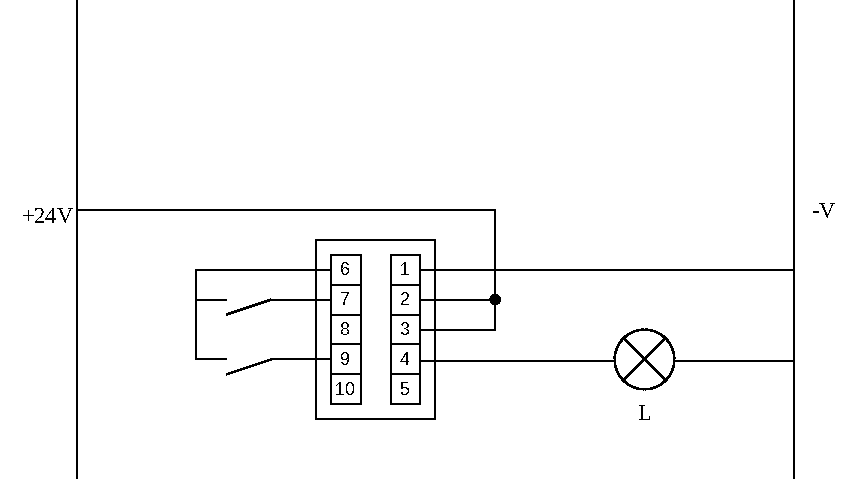
\includegraphics[scale=0.75]{sozai/3.pdf}
  \caption{フローチャート}
\end{figure}

\newpage

\subsection{実験手順}
実験は以下の手順で行う.

\begin{enumerate}
  \item[(1)] 逆運動学(式(2.6),式(2.12)~式(2.14))を計算するエクセルファイルを作成し,表5.2に記された手先位置から関節角度を計算する.数値は小数点第1位まで表記するものとする.
  \item[(2)] 初期位置,No.1~3,初期位置の順に手先位置が到達するようにオンラインティーチングを実行する.
  \item[(3)] 記録した動作をプレイバックする.プレイバックの様子は撮影する.
\end{enumerate}

\begin{table}[h]
  \centering
  \caption{手先位置}
  \begin{tabular}{|c|c|c|c|}
    \hline
    Position No. & $x$ [mm] & $y$ [mm] & $z$ [mm] \\ \hline
    \hline
    1            & 168.1    & 168.1    & 368.8    \\ \hline
    2            & 210.6    & 210.6    & 196.1    \\ \hline
    3            & 541.3    & 0        & 182.8    \\ \hline
  \end{tabular}
\end{table}


\subsection{実験結果}
表5.3に逆運動学の計算結果を示す.また,図5.2に,手先位置がPosition No.2からNo.3に移動した際の経路の模式図を示す.

\begin{table}[h]
  \centering
  \caption{各関節角度の計算結果}
  \begin{tabular}{|c|c|c|c|}
    \hline
    Position No. & $\theta_1$ [deg] & $\theta_2$ [deg] & $\theta_3$ [deg] \\ \hline
    \hline
    1            &                  &                  &                  \\ \hline
    2            &                  &                  &                  \\ \hline
    3            &                  &                  &                  \\ \hline
  \end{tabular}
\end{table}

\subsection{考察}
次に,実行結果の考察を述べる.
 \newpage

%% !TEX root = main.tex

\section{実験2-1:画像処理実験}

\subsection{実験概要}
本実験では,手先に装着したRGB-Dカメラから取得した画像を処理し,
対象物体の検出および3次元位置情報の取得を実験する.
マニピュレータの卓上には,右角度の積み木(赤色,青色,黄色)および収納台が設置されており,
実験では積み木および各収納位置を対象に実験を行う.

\subsection{実験手順}
実験手順は以下の手順で行う.

\begin{enumerate}
  \item[(1)] 卓上に積み木を1個設置し,卓上の目盛りから各物体の$0^{\circ}xy$座標を直接計測し,記録する.
  \item[(2)] Pythonの開発環境Spyderを起動し,画像処理プログラムから空間フィルタリングをOFFにする.
  \item[(3)] 画像処理プログラムを実行後,マニピュレータの制御用ソフトウェアを用いてマニピュレータを手動操作し,画像に積み木が現れる位置まで手先を移動する.この際,手先の位置姿勢を記録する.
  \item[(4)] ヒストグラムを参考にしながら積み木のHSV色空間のしきい値(最大値,最小値)を設定し,記録する.また,スクリーンショット等を用いて,画像処理結果を記録する.
  \item[(5)] 得られた3次元位置情報を記録する.
  \item[(6)] 「平均化フィルタ」,「ガウシアンフィルタ」,「メディアンフィルタ」,「双方向フィルタ」において,それぞれ(1)~(5)を繰り返す.
  \item[(6)] 残りの積み木および収納位置を適所について,(1)~(6)を繰り返す.
  \item[(7)] 式(3.1)を用いて,座標変換を行い,物体の3次元位置をグローバル座標系で表現するエクセルファイルを作成し,計算する.
\end{enumerate}

\subsection{実験結果}
表6.1~表6.3に実験結果を示す.図6.1には,実位置と計測位置の誤差をまとめた図を示す.

\begin{table}[h]
  \centering
  \caption{積み木(赤)の結果}
  \begin{tabular}{|c|c|c|c|c|c|}
    \hline
                                                      & フィルタ無           & 平均フィルタ        & ガウシアンF         & メディアンF         & 双方向フィルタ      \\ \hline
    \hline
    実位置 ($x_{0}^{\circ}, y_{0}^{\circ}$) [mm]      & 488.5 ,-130.0        & 0                   & 0                   & 0                   & 0                   \\ \hline
    手先位置 ($x_{e}^{\circ}, y_{e}^{\circ}, z$) [mm] & 401.1 , 0.0 , 418.2  & 0                   & 0                   & 0                   & 0                   \\ \hline
    手先姿勢 (R, P, Y) [deg]                          & 180, 0 , 0           & 0                   & 0                   & 0                   & 0                   \\ \hline
    H(max, min)                                       & (3,0)                & (10,0)              & (10,0)              & (10,0)              & (10,0)              \\ \hline
    S(max, min)                                       & (255,60)             & (232,61)            & (255,60)            & (255,60)            & (255,60)            \\ \hline
    V(max, min)                                       & (255,0)              & (255,0)             & (255,0)             & (255,0)             & (255,95)            \\ \hline
    計測位置 ($x_{e}^{\circ}, y_{e}^{\circ}, z$) [mm] & (85.1 , 120.1 , 371) & (84.5,130.3,379.9)  & (85.0,128.6,377.9)  & (84.3,124.3,375.9)  & (85.0,126.9,375.9)  \\ \hline
    計測位置 ($x_{0}^{\circ}, y_{0}^{\circ}, z$) [mm] & (486.2,-120.1,47.2)  & (485.6,-130.3,38.3) & (486.1,-128.6,40.3) & (485.4,-204.3,42.3) & (486.1,-126.9,42.3) \\ \hline
  \end{tabular}
\end{table}

\begin{table}[h]
  \centering
  \caption{積み木(青)の結果}
  \begin{tabular}{|c|c|c|c|c|c|}
    \hline
                                                      & フィルタ無          & 平均フィルタ        & ガウシアンF         & メディアンF         & 双方向フィルタ      \\ \hline
    \hline
    実位置 ($x_{0}^{\circ}, y_{0}^{\circ}$) [mm]      & 588.5 ,-130.0       & 0                   & 0                   & 0                   & 0                   \\ \hline
    手先位置 ($x_{e}^{\circ}, y_{e}^{\circ}, z$) [mm] & 401.1 , 0.0 , 418.2 & 0                   & 0                   & 0                   & 0                   \\ \hline
    手先姿勢 (R, P, Y) [deg]                          & 180, 0 , 0          & 0                   & 0                   & 0                   & 0                   \\ \hline
    H(max, min)                                       & (160,140)           & (160,140)           & (160,140)           & (160,140)           & (160,140)           \\ \hline
    S(max, min)                                       & (255,60)            & (255,60)            & (255,60)            & (255,60)            & (255,60)            \\ \hline
    V(max, min)                                       & (255,0)             & (255,0)             & (255,0)             & (255,0)             & (255,0)             \\ \hline
    計測位置 ($x_{e}^{\circ}, y_{e}^{\circ}, z$) [mm] & (181.6,128.1,374.9) & (182.7,131.5,377.9) & (182.1,129.7,375.9) & (182.4,129.0,375.9) & (180.7,127.4,375.9) \\ \hline
    計測位置 ($x_{0}^{\circ}, y_{0}^{\circ}, z$) [mm] & (582.7,-128.1,43.3) & (583.1,-131.5,40.3) & (583.2,-129.7,42.3) & (583.5,-129.0,42.3) & (581.8,-127.4,42.3) \\ \hline
  \end{tabular}
\end{table}

\begin{table}[h]
  \centering
  \caption{積み木(黄)の結果}
  \begin{tabular}{|c|c|c|c|c|c|}
    \hline
                                                      & フィルタ無          & 平均フィルタ        & ガウシアンF         & メディアンF         & 双方向フィルタ      \\ \hline
    \hline
    実位置 ($x_{0}^{\circ}, y_{0}^{\circ}$) [mm]      & 388.5 ,-130.0       & 0                   & 0                   & 0                   & 0                   \\ \hline
    手先位置 ($x_{e}^{\circ}, y_{e}^{\circ}, z$) [mm] & 401.1 , 0.0 , 418.2 & 0                   & 0                   & 0                   & 0                   \\ \hline
    手先姿勢 (R, P, Y) [deg]                          & 180, 0 , 0          & 0                   & 0                   & 0                   & 0                   \\ \hline
    H(max, min)                                       & (50,30)             & (50,30)             & (50,30)             & (50,30)             & (50,30)             \\ \hline 
    S(max, min)                                       & (255,60)            & (255,60)            & (255,60)            & (255,60)            & (255,60)            \\ \hline
    V(max, min)                                       & (255,0)             & (255,0)             & (255,0)             & (255,0)             & (255,0)             \\ \hline
    計測位置 ($x_{e}^{\circ}, y_{e}^{\circ}, z$) [mm] & (-12.3,119.9,365.9) & (-15.0,124.7,370.9) & (-13.0,121.9,366.9) & (-13.0,117.2,365.9) & (-13.0,121.2,365.9) \\ \hline
    計測位置 ($x_{0}^{\circ}, y_{0}^{\circ}, z$) [mm] & (338.8,-119.9,52.3) & (386.1,-124.7,47.3) & (388.1,-121.9,51.3) & (388.1,-117.2,52.3) & (-13.0,121.2,365.9) \\ \hline
  \end{tabular}
\end{table}
\newpage

次に,図6.2に赤ブロックのフィルタ後の画像を示す.

\subsection{考察}
実位置と計測結果の誤差について,考察を行う.

\section{実験2-2:3次元位置計測と物体の把持収納実験}

\subsection{実験概要}
本実験では,手先に装着したRGB-Dカメラから把持物体および収納位置の3次元位置情報を取得し,
物体の把持および収納する実験を行う.図7.1に実験環境の模式図を示す.マニピュレータの卓上には,
把持する五角形の積み木(赤色,青色,黄色)と収納位置用の積み木(黄,青,緑)が置かれている.
マニピュレータは五角形形の積み木を検出・把持して収納位置に配置する動作を行う.

\subsection{実験手順}
実験手順は以下の手順で行う.

\begin{enumerate}
  \item[(1)] 卓上に積み木を3個、収納台座をすべて無造作に配置する.
  \item[(2)] Pythonの開発環境Spyderを起動し,実験3において最も優れた結果となった空間フィルタリングを選択する.
  \item[(3)] 画像処理プログラムを実行後,マニピュレータの制御用ソフトウェアを用いてマニピュレータを手動操作し,画像に各物体が現れる位置まで手先を移動する.この際,手先の位置姿勢を記録する.
  \item[(4)] 実験3で記録したHSV色空間のしきい値を設定し,各物体の検出を行う.また,実験3で作成したエクセルを用いて,各物体の3次元位置をグローバル座標系で表現する.
  \item[(5)] マニピュレータの制御用ソフトウェアを用いて,手先位置の数値指定によるオンラインティーチングを行う.動作は,赤積み木の把持収納,青積み木の把持収納,黄積み木の把持収納をすべて連続で行う.ただし,手先の姿勢$(R, P, Y) = (180, 0, 0)$ [deg]とし,手先の$0^{\circ}$位置を80[mm](把持時),110[mm](収納時)とすること.また,動作の様子を動画撮影する.
\end{enumerate}

\subsection{実験結果}
表7.1に実験結果を示す.また,図7.2にマニピュレータが積み木を把持・収納する様子を示す.

\begin{table}[h]
  \centering
  \caption{物体の位置}
  \begin{tabular}{|c|c|c|c|c|c|c|}
    \hline
                                                      & 赤積木 & 青積木 & 黄積木 & 赤収納              & 青収納              & 黄収納              \\ \hline
    \hline
    手先位置 ($x_{0}^{\circ}, y_{0}^{\circ}, z$) [mm] & 0      & 0      & 0      & 0                   & 0                   & 0                   \\ \hline
    手先姿勢 (R, P, Y) [deg]                          & 0      & 0      & 0      & 0                   & 0                   & 0                   \\ \hline
    計測位置 ($x_{e}^{\circ}, y_{e}^{\circ}, z$) [mm] & 0      & 0      & 0      & (177.7,126.6,375.9) & (88.7,-129.5,372.9) & (-5.7,-128.8,365.9) \\ \hline
    計測位置 ($x_{0}^{\circ}, y_{0}^{\circ}, z$) [mm] & 0      & 0      & 0      & (578.8,-126.6,42.3) & (489.9,129.545.3)   & (395.4,128.852.3)   \\ \hline
    成功                                              & 成功   & 成功   & 成功   & 成功                & 成功                & 失敗                \\ \hline 
    
  \end{tabular}
\end{table}

\subsection{考察}
次に,考察を行う.


%%%%%%%%%%%%%%%%%%%%%%%%%%%%%%%%%%%%%%%%%%%%%%%%%%%%%%%%%%%%%%%
\section{課題}

\subsection{逆運動学の導出}
課題:式(2.6),式(2.12)~式(2.14)を導出せよ.手書き可.
ただし,枠や枠内の文章は報告書に記載不要とする.参考文献は報告書最後の参考文献の欄に記載すること.

\subsection{回転行列とオイラー角の変換式}
課題:式(2.17)~式(2.20)を導出せよ.手書き可.ただし,枠や枠内の文章は報告書に記載不要とする.
参考文献は報告書最後の参考文献の欄に記載すること.

\subsection{空間フィルタリング}
「平均化フィルタ」,「ガウシアンフィルタ」,「メディアンフィルタ」,
「双方向フィルタ」の特徴についてそれぞれ100〜200字程度で説明せよ.
ただし,枠や枠内の文章は報告書に記載不要とする.参考文献は報告書最後の参考文献の欄に記載すること.

\subsection{色空間}
RGB色空間とHSV色空間について,それぞれ100〜200字程度で説明せよ.ただし,
枠や枠内の文章は報告書に記載不要とする.参考文献は報告書最後の参考文献の欄に記載すること.

\subsection{ロボットビジョンの実用例}
ステレオカメラ(単眼カメラでもよい)とロボットマニピュレータを統合することで
可能となる作業の実用例を1例以上調査し,それぞれ200字程度で説明せよ.
ただし,枠や枠内の文章は報告書に記載不要とする.参考文献は報告書最後の参考文献の欄に記載すること.

 \newpage

% !TEX root = main.tex

%%%%%%%%%%%%%%%%%%%%%%%%%%%%%%%%%%%%%%%%%%%%%%%%%%%%%%
\section{実験目的}
%%%%%%%%%%%%%%%%%%%%%%%%%%%%%%%%%%%%%%%%%%%%%%%%%%%%%%
制御系設計には
\begin{itemize}
  \item 運動方程式や回路方程式などから制御対象のモデル(微分方程式,伝達関数など)を導出する
  \item モデルに含まれるパラメータを実験により決定する(パラメータ同定)
  \item 制御対象の出力(制御量)を所望の値にするような制御対象の入力(操作量)を決めるためにコントローラの設計を行う
\end{itemize}
というモデリングの作業と
\begin{itemize}
  \item 制御対象の出力(制御量)を所望の値にするような制御対象の入力(操作量)を決めるためにコントローラの設計を行う
\end{itemize}
というコントローラ設計の作業が含まれる.
本実験では,平面上に回転するアームの角度制御を例として,制御系設計の一連の流れを習得することを
目的としている.

\section{ロボットアーム実験装置の概要と制御目的}

\subsection{ロボットアーム実験装置}

図 2.1 に示すように,ロボットアーム実験装置はアームが水平にして DC モータにより回転するようになっている.
DC モータを駆動させるためにパソコン上で計算された指令電圧は,I/O ボード "Q8-USB" により D/A 変換され,
アンプを介して DC モータに入力される.
さらに,アームの角度はシャフトに取り付けてあるポテンショメータによって角度として検出され,
I/O ボード "Q8-USB" により A/D 変換されて後,パソコンに取り込まれている.

\subsection{アクチュエータと D/A 変換}

コンピュータから出力される指令電圧はデジタル値であるため,D/A 変換によってアナログ値に変換される
(図 2.2 に示す).アナログ周期ごとに一定値のアクションに変換してからアンプに加える必要がある.
指令電圧の I/O ボード "Q8-USB" による D/A 変換には,16 ビットが使われており,
分解能は \(0.30518 [V] = (\pm 10 - (-10))/2^{16} \)[V] の刻み幅である.

\begin{figure}[h]
  \centering
  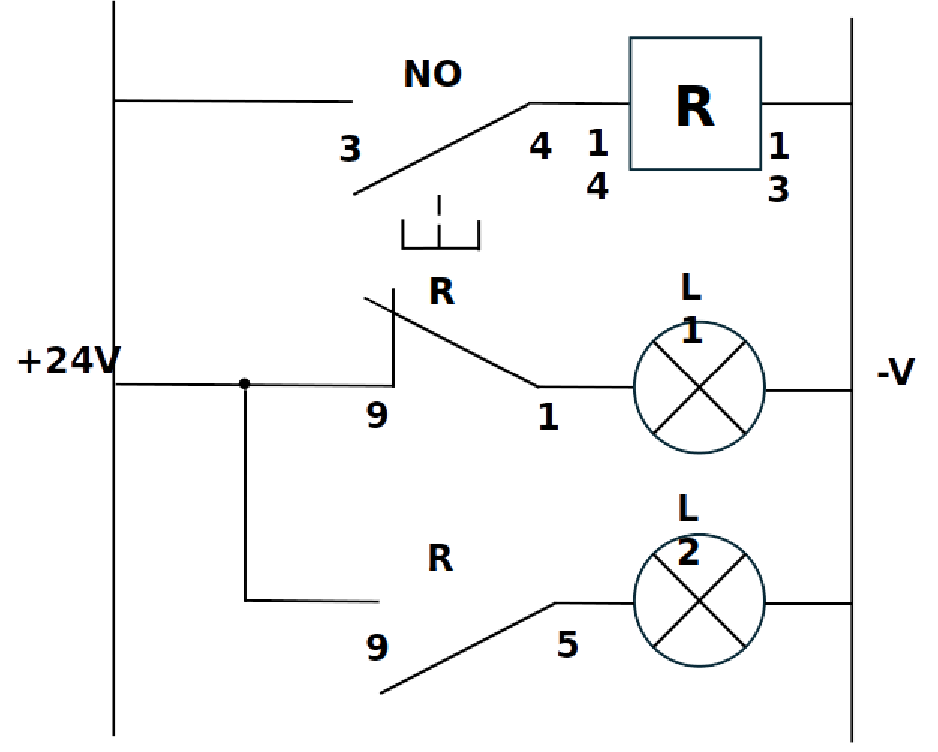
\includegraphics[scale=0.4]{sozai/1.pdf}
  \caption{ロボットアーム実験装置}
\end{figure}

\begin{figure}[h]
  \centering
  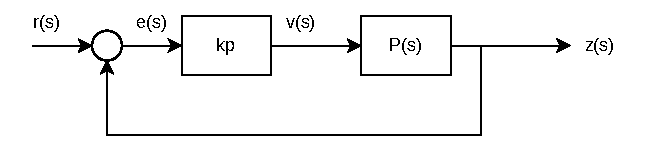
\includegraphics[scale=0.65]{sozai/2.pdf}
  \caption{制御対象のブロック線図}
\end{figure}

\subsection{センサと A/D 変換}

本実験装置では,ロボットアームの角度を検出するためのセンサにポテンショメータが用いられている.
ポテンショメータは可変抵抗であり角度に比例した電圧(アナログ量)\(V_s\)[V] を返す.
センサの出力電圧とロボットアームの角度との関係は,1 [V] あたり \(-35\) [deg] であり,
\(-175 \sim 175\) [deg] の角度を検出可能である.

コンピュータでこのセンサ電圧 \(V_s(t) \)[V] を利用するには,
A/D 変換によってアナログ量をサンプリング周期 [s] でディジタル量に変換する必要がある.
A/D 変換では,\(V_s(kh) \)[V] のように \(V_s(t)\) を横軸(時間軸)方向に離散化する標本化の作業と,
\(V_s(kh)\) を縦軸方向に離散化する量子化の作業を行う.
本実験装置の I/O ボード "Q8-USB" 上の A/D 変換部はレンジ:\(\pm 5 \)[V] または \(\pm 10 \)[V],
分解能:16 ビットである.本実験では,レンジを \(\pm 5 \)[V] に設定しているため,
約 0.15259 [mV] =\( (\pm 5 - (-5))/2^{16} \)[V] の刻み幅(量子化サイズ)で量子化することになる.

\subsection{制御目的と P 制御}

本実験では,ロボットアームの回転角度を所望の角度ですばやく止める角度制御を考える.
角度制御を実現するために考えられる最も単純な方法は,
\begin{itemize}
  \item 目標角 \( \theta_{\text{ref}}(t) \) と回転角 \( \theta(t) \) の差(偏差と呼ぶ)を計算
  \item その差が正(負)に大きければ正(負)の大きな電圧 \(v(t)\) を加える
  \item 正(負)に小さければ正(負)の小さな電圧 \(v(t)\) を加える
\end{itemize}
という方法である.このように偏差 \(e(t) = \theta_{\text{ref}}(t) - \theta(t)\) 
に比例した電圧 \(v(t)\) を加えるような制御方法をP制御(比例制御)という.また,
\begin{equation}
  v(t) = k_{\mathrm{P}} e(t) \quad \Longleftrightarrow \quad v(s) = k_{\mathrm{P}} e(s)
\end{equation}
という形式のコントローラをPコントローラと呼ぶ.


\begin{figure}[h]
  \centering
  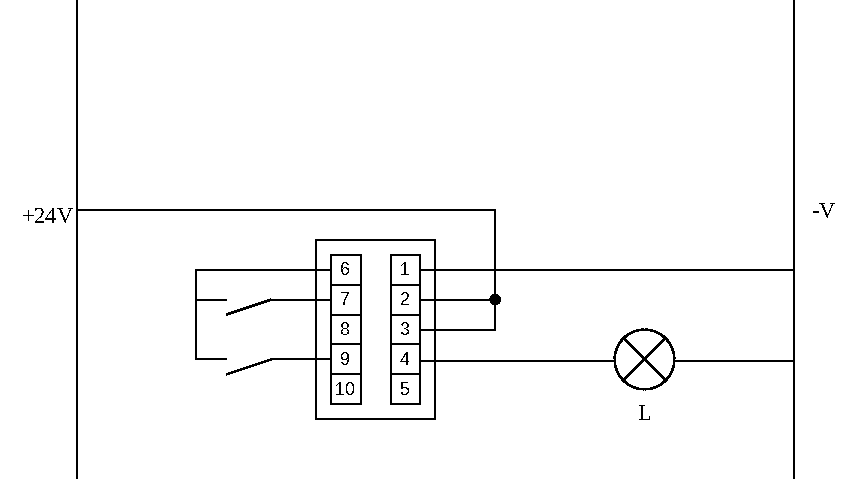
\includegraphics[scale=1]{sozai/3.pdf}
  \caption{P制御}
\end{figure}

\begin{figure}[h]
  \centering
  \includegraphics[scale=1]{sozai/group03/ad_da/ad_da_conv-crop.pdf}
  \caption{P制御}
\end{figure}

\subsection{PI 制御}
P 制御では様々な要因でステップ状の目標値に対する定常偏差が生じることがある.
この定常偏差を零にするためには,コントローラに積分動作 \( k_I /s \) を含ませればよく,

\begin{equation}
  v(t) = k_{\mathrm{P}} e(t) + k_I \int_{0}^{t} e(\tau) d\tau \quad \Longleftrightarrow \quad v(s) = \left( k_{\mathrm{P}} + \frac{k_I}{s} \right)e(s)
\end{equation}

という形式のコントローラを PI コントローラと呼ぶ.


\section{実験 1 -- A/D, D/A 変換の動作確認と P, PI 制御 --}

\subsection{実験装置のセッティング}
ロボットアーム実験装置が図~3.1 のように結線されていることを確認する.


\begin{figure}[h]
  \centering
  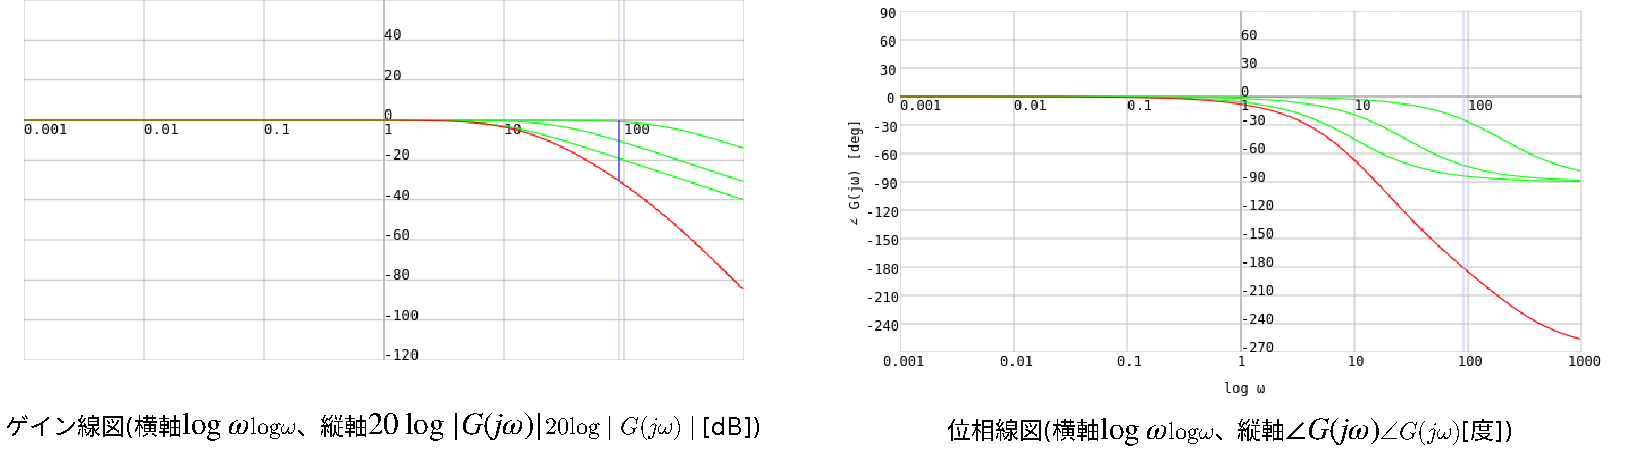
\includegraphics[scale=0.8]{sozai/4.pdf}
  \caption{ロボットアーム実験装置の結線}
\end{figure}

\subsection{D/A 変換とアクチュエータの動作確認}
\begin{enumerate}
  \item D/A 変換の動作確認をするために図~3.2 の Simulink モデル ``da\_conv.slx'' を作成する.
        保存場所は D:\#student\_5S\#group01\#da (``01'' は班の番号であり,
        2 班なら ``01'' を ``02'' に読み替え)とする.Simulink モデルをビルドし,
        エラーがないことを確認した後,
        \begin{lstlisting}
  >> print -s -dpdf da_conv.pdf    
  \end{lstlisting}
        と入力して Simulink モデル ``da\_conv.slx'' の pdf ファイル ``da\_conv.pdf'' を生成する.
        さらに,生成した pdf ファイルの余分な空白を取り除くため,``da\_conv.pdf'' をデスクトップ上の
        ``bcpdfcrop-multi.bat'' にドラッグする.その結果,``da\_conv-crop.pdf'' が生成される.
        
        なお,QuaRC により利用できる Simulink ブロック HIL Initialize や HIL Write Analog については
        補足 1.1,パラメータ設定については補足 1.2, 1.3, ビルドと実行の方法については補足 1.4 を参照すること
        (別紙「補足事項:QuaRC の使用方法」).
  \item Simulink モデル “da\_conv.slx” のブロック Manual Switch を “Constant” 側にする.Simulink モデルの実行を開始すると,DC モータに一定の電圧が加わり,アームが一定速度で回転することを確認せよ.
  \item テスタを Universal Power Module の “OUT” と “GND” に接続する.図 3.2 の Constant ブロックを表 3.1 のように設定したときのテスタの測定値およびアームの動作を観測し,表 3.1 を完成せよ.
  \item Universal Power Module の “To Load” に接続されているケーブルの DC モータ側を取り外し,オシロスコープを Universal Power Module の “OUT” と “GND” に接続する.(オシロスコープの電圧レンジは 5 [V/DIV],時間レンジは 2 [msec/DIV] に設定する.\\
        \quad Simulink モデル “da\_conv.slx” のブロック Manual Switch を “Sine Wave” 側にする.ブロック “Sine Wave” の周波数を “pi/0.008” [rad/s],振幅を “5”,“10”,“15” と設定したとき,D/A 変換された電圧をオシロスコープで観測し,デジタルカメラで撮影せよ(付録 A.1 の 図 A.1 を参照).
\end{enumerate}

\subsubsection{実験結果}
以下に結果を示す.

\begin{figure}[h]
  \centering
  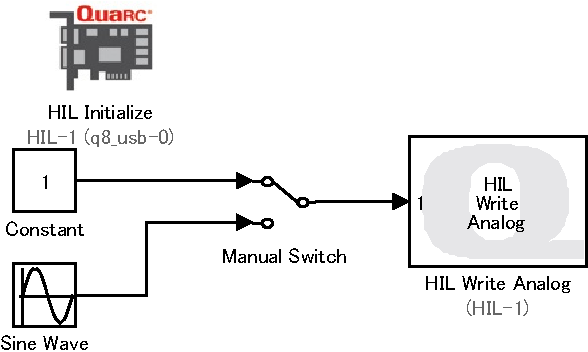
\includegraphics[scale=1]{sozai/da_conv-crop.pdf}
  \caption{da\_conv}
\end{figure}

\newpage

\begin{table}[h]
  \centering
  \caption{D/A 変換の動作確認とアームの回転方向}
  \begin{tabular}{|c|c|c|}
    \hline
    ブロック Constantの設定値 [V] & テスタによる測定値 [V] & 回転方向 (時計回り,反時計回り,静止) \\ \hline
    -5                            & -5                     & cww                                 \\ \hline
    -2.5                          & -2.494                 & cww                                 \\ \hline
    -1                            & -0.994                 & csww                                \\ \hline
    -0.5                          & -0.495                 & cww                                 \\ \hline
    0                             & \(4.7×10^{-3}\)        & 静止                                \\ \hline
    0.5                           & 0.504                  & cw                                  \\ \hline
    1                             & 1.003                  & cw                                  \\ \hline
    2.5                           & 2.502                  & cw                                  \\ \hline
    5                             & 5                      & cw                                  \\ \hline
  \end{tabular}
\end{table}

\begin{figure}[h]
  \centering
  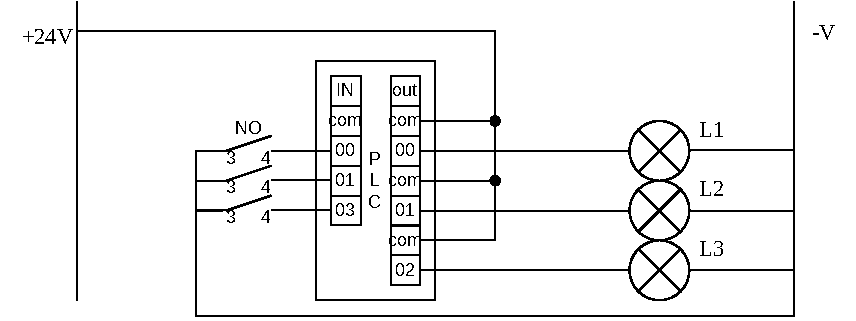
\includegraphics[scale=2]{sozai/5.pdf}
  \caption{オシロスコープ a=5,b=10,c=15}
\end{figure}

\subsubsection{実験考察}
da\_convにより設定値[v]がマイナスのとき反時計回り(ccw),プラスのときに時計回り(cw)となることが
表3.1よりわかる.また,出力値をテスターで計測したところほぼ設定値と同程度の電圧が測定できた.
これによりconstantの値をそのまま出力していることがわかる.

次にオシロスコープでは,振幅を5,10,15と変化させ観測したが,すべて16個の線により表されていた.
これは以下の式よりわかる.

周波数 \( f \) を \( \omega = \frac{\pi}{0.008} \, \text{[rad/s]} \) の場合に求めるには,
角周波数 \( \omega \) と周波数 \( f \) の関係を使用する.
\begin{equation}
  \omega = 2\pi f
\end{equation}
この式からより

\begin{equation}
  f = \frac{\omega}{2\pi}
\end{equation}

となり,角周波数 \( \omega = \frac{\pi}{0.008} \) の場合,

\begin{equation}
  f = \frac{\frac{\pi}{0.008}}{2\pi} = \frac{1}{2 \times 0.008} = \frac{1}{0.016} = 62.5 \, \text{[Hz]}
\end{equation}

つまり,角周波数が \( \frac{\pi}{0.008} \, \text{[rad/s]} \) の場合,
周波数 \( f \) は \( 62.5 \, \text{[Hz]} \) となる.
よって
\begin{equation}
  T = \frac{1}{f}
\end{equation}
\begin{equation}
  T = \frac{1}{62.5} = 0.016 \, \text{[s]}
\end{equation}

したがって,周期 \( T \) は \( 0.016 \, \text{[s]} \) となる.
サンプリング周期が1[ms]のため,16個の線により表された.


\subsection{A/D変換とセンサの動作確認}
\begin{enumerate}
  \item A/D変換の動作確認をする図3.3のSimulinkモデル“ad\_conv.slx”を作成する.保存場所は D:\#student\_5S\#group01\#ad とする.ビルドしてエラーがないことを確認した後,printコマンドにて“ad\_conv.pdf”という名前のpdfファイルを生成し,デスクトップ上の“bcpdfcrop-multi.bat”により余白を取り除く.
  \item テスタをUniversal Power Moduleの“S1”と“GND”に接続し,アームを±45度に動かす(目測で良い).そのときのDisplay値とテスタの値を観測し,表3.2を完成せよ.
  \item 表3.2の結果から,センサ電圧1[V]あたりの角度変位を求めよ(符号に注意).
        \begin{equation}
          \text{センサ電圧 1 [V] あたりの角度変位} = {\large\textbf{     }} \, \text{[deg]} = {\large\textbf{     }} \, \text{[rad]}
        \end{equation}
  \item アームを1回転させたとき,センサ電圧の範囲をテスタにより測定せよ.
        \begin{equation}
          \text{センサ電圧:最小値} = {\large\textbf{     }} \, \text{[V]} , \quad \text{最大値} = {\large\textbf{     }} \, \text{[V]}
        \end{equation}
\end{enumerate}


\subsubsection{実験結果}
以下に結果を示す.

\begin{figure}[h]
  \centering
  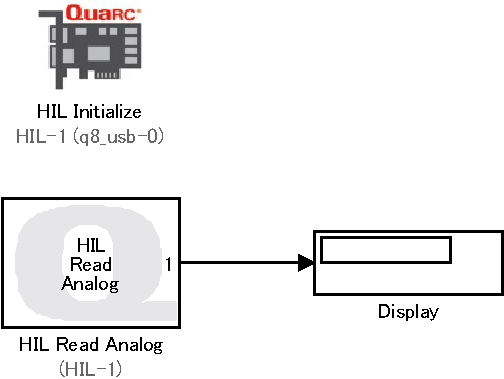
\includegraphics[scale=1]{sozai/ad_conv-crop.pdf}
  \caption{ad\_conv}
\end{figure}

\newpage

\begin{table}[h]
  \centering
  \caption{A/D変換の動作確認(角度:反時計回りが正)}
  \begin{tabular}{|c|c|c|}
    \hline
    アームの回転角度 [deg] & テスタによる測定値 [V]  & Displayによる測定値 [V] \\ \hline
    45                     & {\large\textbf{1.030}}  & {\large\textbf{1.031}}  \\ \hline
    0                      & --                      & --                      \\ \hline
    -45                    & {\large\textbf{-1.520}} & {\large\textbf{-1.521}} \\ \hline
  \end{tabular}
\end{table}

\begin{equation}
  \text{センサ電圧 1 [V] あたりの角度変位} = {\large\textbf{-35.266}} \, \text{[deg]} = {\large\textbf{-0.6155}} \, \text{[rad]}
\end{equation}

\begin{equation}
  \text{センサ電圧:最小値} = {\large\textbf{-4.95}} \, \text{[V]} , \quad \text{最大値} = {\large\textbf{5.05}} \, \text{[V]}
\end{equation}

\subsubsection{実験考察}
この実験では,ポテンショメータを使用し角度を検出した.ポテンショメータはロータリエンコーダなどのパルス信号と異なり,
アナログ電圧を出力する絶対的な位置情報を持つアナログセンサである.
実験では45,−45度のときの電圧を計測し,計90度で2.552[v]変化した.
これにより1[v]あたりの角度変位を求めることができた.
また,式(3.9)より角度の検出範囲を求めることができる.
センサ電圧の範囲は,全体で
\[
  5.05 - (-4.95) = 10 \, \text{[V]}
\]
の変化がある.この電圧範囲に対する角度変位は,1[V]あたりの角度変位を掛けることで計算でき,
\[
  \text{角度の検出範囲} = 10 \, \text{[V]} \times (-35.266 \, \text{[deg/V]}) = -352.66 \, \text{[deg]}
\]
となる.
したがって,ポテンショメータの角度検出範囲は約\(352.66\) [deg]であることがわかる.




\subsection{ロボットアームの表現}

\begin{enumerate}
  \item 以下の動作をするような図3.4のSimulinkモデルを完成させる.
        \begin{itemize}
          \item アンプに加える電圧が $-10 \sim 10 \, [V]$ の範囲を超えないようにする.
          \item コンピュータから正の指令電圧を与えたとき,アームが反時計回りに回転する.
          \item センサ電圧を角度 $[rad]$ で出力する.ただし,この実験のみScopeはdegで表示させる.
          \item 終了時間が8秒となるようにする.
        \end{itemize}
        
        各ブロックのパラメータ設定は各自で考えることとし,完成したSimulinkモデルは“ad\_da\_conv.slx”という名前でディレクトリ \texttt{D:\#student\_5S\#group01\#ad.da} に保存する.ビルドしてエラーがないことを確認した後,printコマンドにて“ad\_da\_conv.pdf”という名前のpdfファイルを生成し,デスクトップ上の“bcpdfcrop-multi.bat”により余白を取り除く.
        
  \item 3.2節(4)で外したケーブルを接続する.
  \item オシロスコープをUniversal Power Moduleの“$S1$”と“$GND$”に接続し,センサ電圧が $0 [V]$ になるように,アームを動かす.
  \item Scopeをダブルクリックして開き,リアルタイムで角度データを観測できるようにする.Scopeのレンジは付録A.1の図A.2に合わせる.設定方法は図3.5に示す.
  \item すべての準備が整ってから“ad\_da\_conv.slx”を実行する.実行終了後,コマンドウィンドウで
        \begin{verbatim}
    >> save ad_da_data t y 
    \end{verbatim}
        と入力し,“ad\_da\_data.mat”という名前のmatファイルでデータを保存する.また,配布するMファイル
        \begin{itemize}
          \item “autoplot\_ad\_da.m”
        \end{itemize}
        を実行することによって,MATLAB上でグラフを作成する.グラフのpdfファイルは自動的に生成される.
\end{enumerate}

\subsubsection{実験結果}
以下に結果を示す.

\begin{figure}[h]
  \centering
  \includegraphics[scale=1]{sozai/ad_da_conv-crop.pdf},
  \caption{ad\_da\_conv}
\end{figure}

\begin{figure}[h]
  \centering
  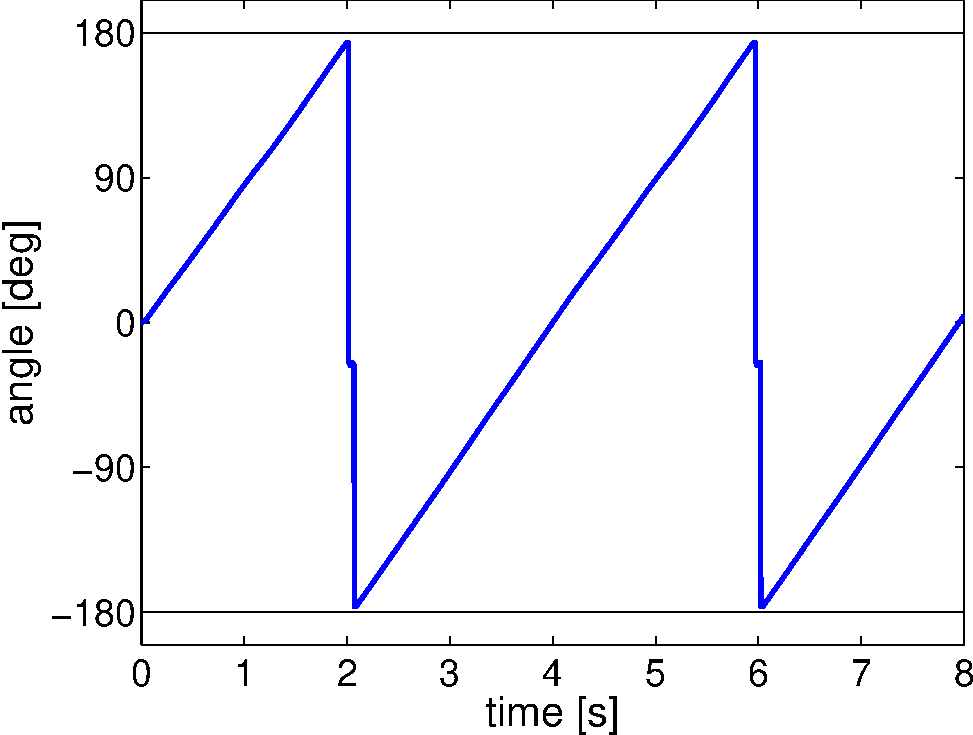
\includegraphics[scale=0.5]{sozai/figure_ad_da-crop.pdf}
  \caption{A/D,D/A変換の動作確認}
\end{figure}

\subsubsection{実験考察}
ポテンショメータには検出可能な範囲に制限があるため,
設定された範囲(ここでは180度)に到達すると,値が再び最小値(-180度)に戻っている.
これは,ポテンショメータが無限に回転するのではなく,
ある範囲内でのみ動作するように設計されているためだと考えられている.

\subsection{P制御}

ここではアームの角度制御のためにPコントローラ
\begin{equation}
  v(t) = k_{\mathrm{P}} \left( \theta^{\text{ref}}(t) - \theta(t) \right) \quad \left( \theta^{\text{ref}}(t) : \text{目標値} , \, \theta(t) : \text{現在の角度} \right)
\end{equation}
を用い,比例ゲイン $k_{\mathrm{P}}$ を大きくするにしたがって過渡特性,定常特性がどのように変化するかを調べる.


\begin{enumerate}
  \item P制御を行うため,図3.6のSimulinkモデル“ex\_pcont.slx”を作成する.モデルはディレクトリD:\#student\_5S\#group01\#pcontに保存する.つぎに,
        \begin{verbatim}
          >> kP = 2;
        \end{verbatim}
        と入力した後,ビルドを行いエラーがないことを確認する.また,“ex\_pcont.pdf”という名前のpdfファイルを生成し,デスクトップ上の“bcpdfcrop-multi.bat”により余白を取り除く.
        
  \item ScopeとScope1を開き,リアルタイムで角度と操作量を観測できるようにする.レンズは付録A.1の図A.3に合わせる.
        
  \item センサ電圧が0 [V]となる位置にアームを動かし,“ex\_pcont.slx”を実行する.実行終了後,
        \begin{verbatim}
          >> save pcont_kP02_data t u y kP
        \end{verbatim}
        と入力し,matファイル“pcont\_kP02.data.mat”にデータを保存する.
        
        同様に,$k_{\mathrm{P}} = 4$, $k_{\mathrm{P}} = 20$と設定して“ex\_pcont.slx”を実行し,実験結果のデータを
        \begin{itemize}
          \item “pcont\_kP04.data.mat” ($k_{\mathrm{P}} = 4$)
          \item “pcont\_kP20.data.mat” ($k_{\mathrm{P}} = 20$)
        \end{itemize}
        という名前のmatファイルに保存する.
        
        最後に,配布するMファイル
        \begin{verbatim}
          >> autoplot_pcont.m
        \end{verbatim}
        を実行することによって,MATLAB上でグラフを作成する.グラフのpdfファイルは自動的に生成される.
\end{enumerate}

\subsubsection{実験結果}
以下に結果を示す.
\begin{figure}[h]
  \centering
  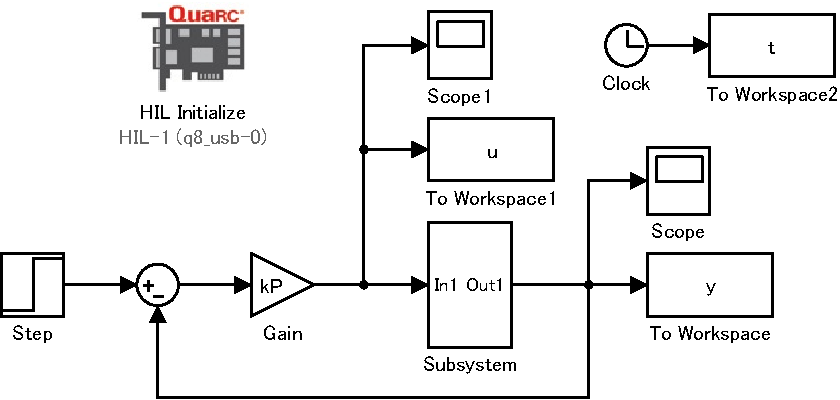
\includegraphics[scale=1]{sozai/ex_pcont-crop.pdf}
  \caption{ex\_pcont}
\end{figure}

\begin{figure}[h]
  \centering
  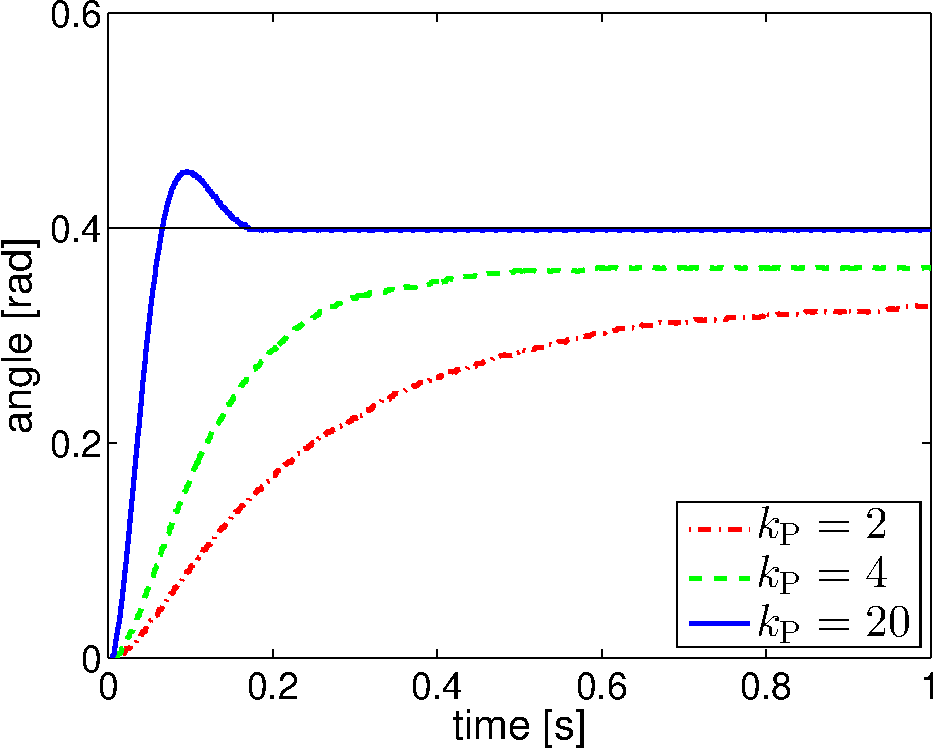
\includegraphics[scale=0.6]{sozai/figure_pcont_angle-crop.pdf}
  \caption{figure\_pcont\_angle}
\end{figure}

\begin{figure}[h]
  \centering
  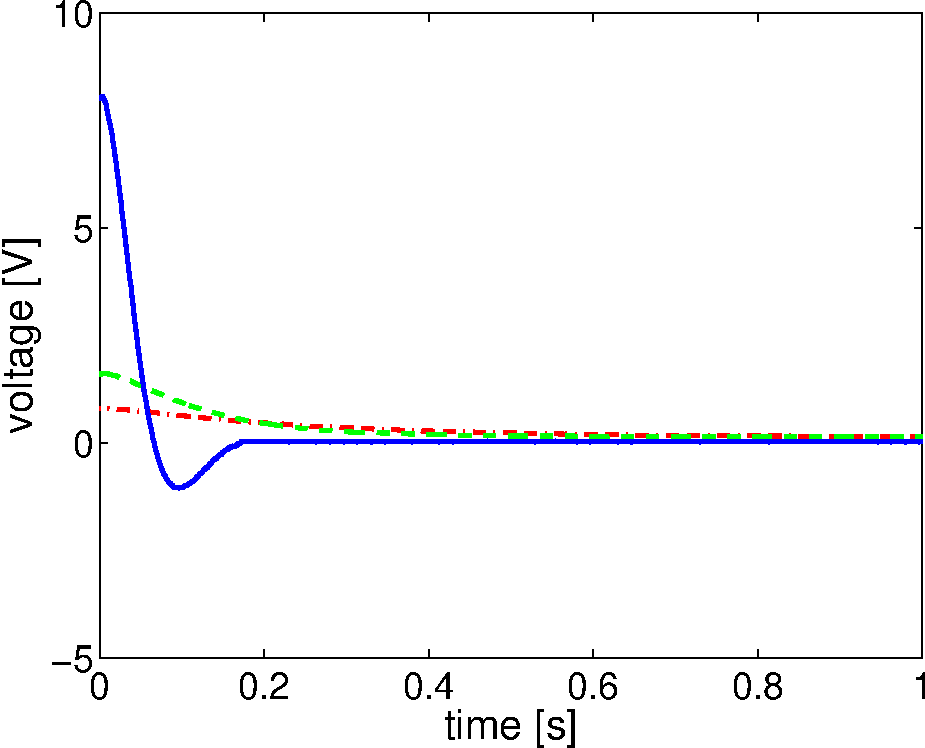
\includegraphics[scale=0.6]{sozai/figure_pcont_volt-crop.pdf}
  \caption{figure\_pcont\_volt}
\end{figure}

\subsubsection{実験考察}
図3.8と図3.9より,比例ゲイン \( k_{\mathrm{P}}\) を増加させると,
過渡特性における立ち上がり時間が短くなり,応答がより速くなることが観察できる.
これは,比例ゲイン \( k_{\mathrm{P}}\) が大きいほど制御系が目標値に迅速に追従しようとするためであり,
その結果として立ち上がり時間が短縮される.
一方で,比例ゲインが大きくなるとオーバーシュートの値も増加する傾向がある.
これは,ゲインが高いことで目標値に達する速度が増加しすぎ,目標値を超過してしまうためである.
また,操作量(入力電圧)の大きさも比例ゲイン \( k_{\mathrm{P}}\) によって増加する.
これは,制御対象が目標値から離れているときに強い制御力が働くためであり,
制御量が過大になりやすい.図3.9に示されるように, \( k_{\mathrm{P}}\) の増加に伴って初期の入力電圧が
大きくなるが,これは目標角度に迅速に追従するために必要な制御信号が大きくなるためである.
次に,定常特性(定常偏差)について考察する.比例制御のみでは,
制御対象に定常偏差が残ることがある.この理由は,比例制御が誤差に比例した制御量を出力するため,
目標値に完全に一致するためには無限大のゲインが必要となるためである.
したがって,有限の \( k_{\mathrm{P}}\)  のもとでは完全に目標値に一致することは難しい.
理論的には,最終値の定理を用いて定常偏差を考察することができる.
入力がステップ応答の場合,最終値の定理より,システムの出力 \( y(t) \) の定常値は以下で与えられる.

\begin{equation}
  \lim_{t \to \infty} y(t) = \lim_{s \to 0} s \cdot Y(s)
\end{equation}

ここで, \( Y(s) \) はシステムの出力のラプラス変換である.
比例制御のみを用いたシステムでは,定常偏差がゼロにならないため,
入力と出力の間に誤差が残る.これは,実機の摩擦や負荷変動などの外乱要因が存在するためでもある.
ポテンショメータやエンコーダのセンサー精度や摩擦力,モータの不間帯などが影響を及ぼし,
理想的な追従が難しい要因ともなっていると考えられる.


\subsection{積分動作の効果(PI制御)}

\begin{enumerate}
  \item PI 制御を行うため,図 3.7 の Simulink モデル ``ex\_picont.slx'' を作成する.モデルはディレクトリ D:\#student.5S\#group01\#picont に保存する.つぎに,
        \begin{verbatim}
        >> kP = 4; kI = 0;
    \end{verbatim}
        と入力した後,ビルドを行いエラーがないことを確認する.また,``ex\_picont.pdf'' という名前の pdf ファイルを生成し,デスクトップ上の ``bcpdfcrop-multi.bat'' により余白を取り除く.
        
  \item Scope と Scope1 を開き,リアルタイムで角度と操作量を観測できるようにする.レンズは付録 A.1 の図 A.4 に合わせる.
        
  \item センサ電圧が 0 [V] となる位置にアームを動かし,``ex\_picont.slx'' を実行する.実行終了後,
        \begin{verbatim}
        >> save picont_kP04_kI00_data t u y kP kI
    \end{verbatim}
        と入力し,mat ファイル ``picont\_kP04\_kI00.data.mat'' にデータを保存する.
        
        比例ゲインを \( k_{\mathrm{P}} = 4 \) に固定し,積分ゲインを \( k_I = 6 \),\( k_I = 12 \) として ``ex\_picont.slx'' を実行し,実験結果のデータを
        \begin{itemize}
          \item ``picont\_kP04\_kI06.data.mat'' \((k_{\mathrm{P}} = 4, k_I = 6)\)
          \item ``picont\_kP04\_kI12.data.mat'' \((k_{\mathrm{P}} = 4, k_I = 12)\)
        \end{itemize}
        という名前の mat ファイルに保存する.最後に,配布する M ファイル ``autoplot\_picont.m'' を実行することによって,MATLAB 上でグラフを作成する.グラフの pdf ファイルは自動的に生成される.
        
  \item 目標値を 0 に設定(Step の最終値を ``0'' に設定)し,また,終了時間を ``inf'' に設定する.比例ゲインを \( k_{\mathrm{P}} = 4 \) に固定し,積分ゲインを \( k_I = 0, k_I = 12 \) として実験を行い,手でアームに力を加えたとき(入力外乱を加えることに相当),反力がどうなるか調べる.
\end{enumerate}

\subsubsection{実験結果}
以下に結果を示す.
\begin{figure}[h]
  \centering
  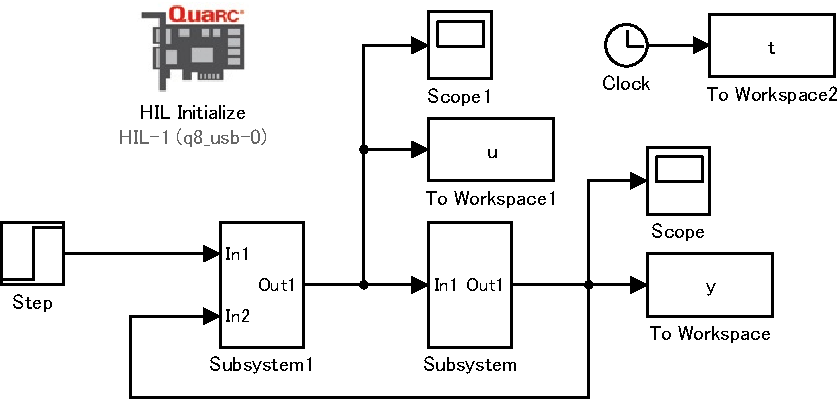
\includegraphics[scale=0.7]{sozai/ex_picont-crop.pdf}
  \caption{ex\_picont}
\end{figure}

\begin{figure}[h]
  \centering
  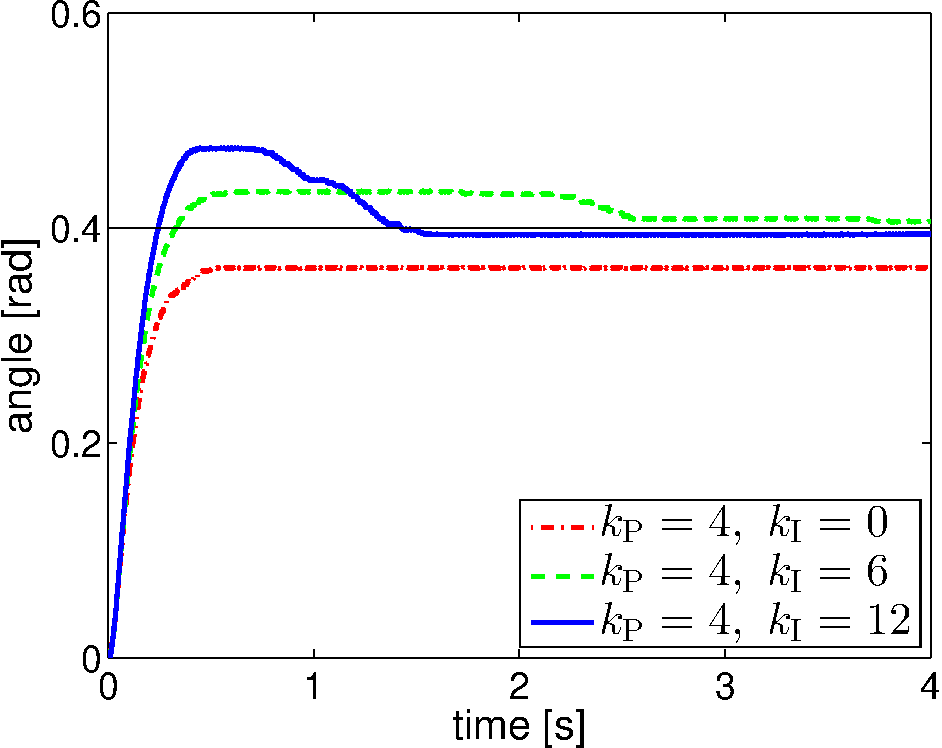
\includegraphics[scale=0.5]{sozai/figure_picont_angle-crop.pdf}
  \caption{figure\_picont\_angle}
\end{figure}

\begin{figure}[h]
  \centering
  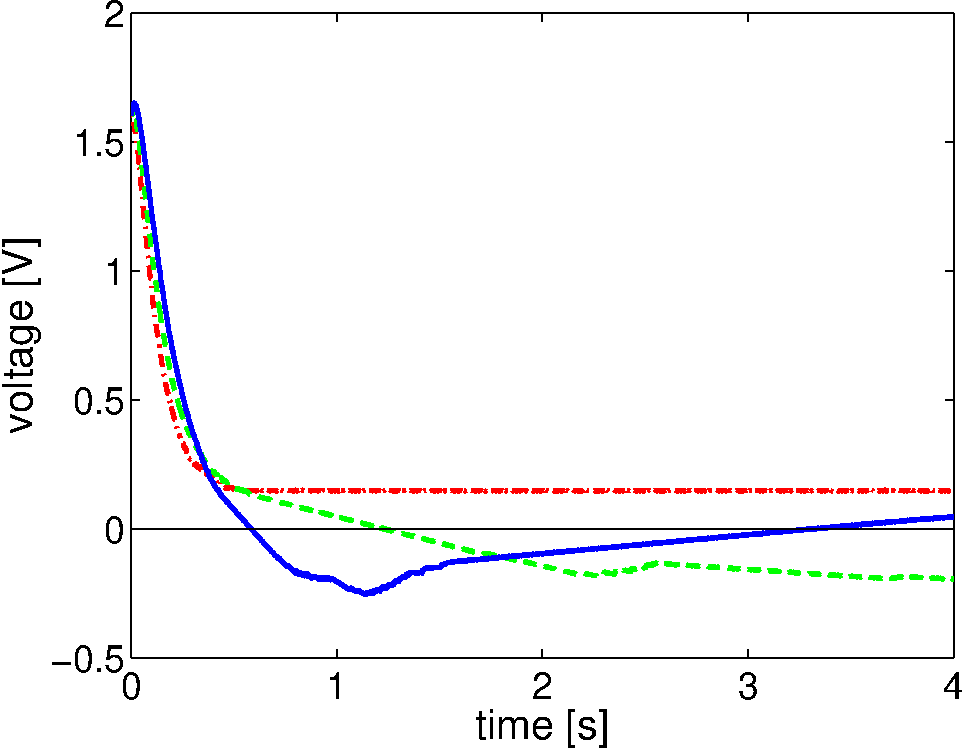
\includegraphics[scale=0.5]{sozai/figure_picont_volt-crop.pdf}
  \caption{figure\_picont\_volt}
\end{figure}

\newpage

\subsubsection{実験考察}
積分動作の導入により,定常偏差が収束したことが図3.11よりわかる.
定常偏差が収束した理由は,積分動作が偏差の累積に基づいて補正を行うためである.
制御系において,積分動作は偏差が存在する限り制御信号を加え続け,
目標値に到達するまでその効果を増大させる.
これにより,定常偏差が時間とともに蓄積されて制御信号として反映され,
結果として定常偏差が収束する形で解消されるため,最終的にシステムは目標値に到達する.
さらに,積分動作による定常偏差の解消は,最終値の定理からも説明できる.
最終値の定理により,システムの出力が時間無限大において収束する値は,
ラプラス変換されたシステムの伝達関数 \( G(s) \) と入力 \( R(s) \) の積の 
\( s \to 0 \) の極限で表される.たとえば,ステップ入力 \( R(s) = \frac{1}{s} \) を用いると,
出力の最終値は次のように表される
\[
  \lim_{t \to \infty} y(t) = \lim_{s \to 0} s \cdot \frac{G(s)}{1 + G(s)H(s)} \cdot \frac{1}{s}
\]
積分動作を持つPI制御系では,伝達関数 \( G(s)H(s) \) に積分項 \(\frac{1}{s}\) が含まれるため,
分母が無限大となり,上記の極限は入力に対して出力が収束することを示す.
これにより,定常偏差はなくなることが保証される.
また,アームに外力が加わった場合,P制御では差分に応じた出力のみで対応するため,
外力に対して定常偏差が残りやすい.しかし,PI制御では偏差が積分され,
外力が加わり続ける限り制御出力も増大するため,徐々に出力が大きくなり,
外力に打ち勝って目標値に収束する挙動が見られる.

 \newpage

% !TEX root = main.tex

\section{モデルに基づく改良型PID制御}

ここではまず,ロボットアームのモデリングについて説明する.
ついで,このモデルに基づいて部分的モデルマッチング法(北森の方法)による
改良型PIDコントローラのパラメータ調整について説明する.

\subsection{ロボットアームのモデリング}
\subsubsection{運動方程式と伝達関数}
ロボットアームの運動方程式は
\begin{equation}
  J \ddot{\theta}(t) = -c \dot{\theta}(t) + \tau(t)
  \tag{4.1}
\end{equation}
で与えられる.ただし,$\tau(t)$ [N·m]: アームの回転軸に加わるトルク,$c$: アームの回転軸の粘性摩擦係数,$J$ [kg·m²]: アームの慣性モーメントである.(4.1)式に,
DC モータ,アンプの特性式やギア比を考慮すると,ロボットアームシステム全体の数学モデルは,
\begin{equation}
  \ddot{\theta}(t) = -a \dot{\theta}(t) + b v(t)
  \tag{4.2}
\end{equation}
という形式となる.ここで,$v(t)$ [V]: モータを駆動させるための指令電圧,
$a, b$: アーム,DC モータ,アンプの特性やギア比に関わるパラメータである.

角度制御を考えた場合,制御量は $\theta(t)$,操作量は $v(t)$ であるから,
$v(s) = \mathcal{L}[v(t)]$ から $\theta(s) = \mathcal{L}[\theta(t)]$ への伝達関数 
$P(s)$ は

\begin{equation}
  P(s) = \frac{\theta(s)}{v(s)} = \frac{b}{s(s+a)}
  \tag{4.3}
\end{equation}

となる.

\subsubsection{パラメータ同定}

(4.3)式に含まれるパラメータ $a$, $b$ は測定器で測ることができない未知パラメータである.
そこで,実験によりパラメータ同定を行う.
\begin{align}
  y_d(t) & = \dot{\theta}(t)
\end{align}とすると(4.2)式は    
\begin{align}                                                                    
  y_d(t) & = -a y_d(t) + b v(t) 
\end{align}となるから,    
\begin{align}                                                                             
  v(s) & = \mathcal{L}[v(t)]
\end{align} から
\begin{align}  
  y_d(s) = \mathcal{L}[y_d(t)]
\end{align}への伝達関数 \(P_d(s)\) は1次遅れ要素
\begin{equation}
  P_d(s) = \left( \frac{y_d(s)}{v(s)} \right) = \frac{b}{s + a} \tag{4.5}
\end{equation}
となる.(4.5)式を1次遅れ要素の標準形で表すと
\begin{equation}
  P_d(s) = \frac{K}{1 + Ts}, \quad T = \frac{1}{a}, \quad K = \frac{b}{a} \tag{4.6}
\end{equation}

であるから,$v(t) = 1$ [V] を加えたときの角速度(単位ステップ応答) $y_d(t) = \dot{\theta}(t)$ は図 4.3 のようになる.
したがって,時定数 $T$,ゲイン $K$ を求めれば,未知パラメータ $a, b$ が次式のように定まる.
\begin{equation}
  a = \frac{1}{T}, \quad b = Ka = \frac{K}{T} \tag{4.7}
\end{equation}

\subsection{部分的モデルマッチング法によるPIDコントローラの設計}
\subsubsection{P-D制御(微分先行型PD制御)}
P-D コントローラ(微分先行型PD コントローラ)
\begin{equation}
  v(t) = k_{\mathrm{P}} e(t) - k_D \frac{d}{dt} \theta(t) \quad \Longleftrightarrow \quad v(s) = k_{\mathrm{P}} e(s) - k_D s \theta(s)
\end{equation}
を用いると,(4.5),(4.8) 式より $\theta^{\text{ref}}(s)$ から $\theta(s)$ への伝達関数は2 次遅れ要素
\begin{equation}
  T(s) = \frac{\omega_n^2}{s^2 + 2 \zeta \omega_n s + \omega_n^2}, \quad \omega_n = \sqrt{b k_{\mathrm{P}}}, \quad \zeta = \frac{a + b k_D}{2 \omega_n}
\end{equation}
となる.したがって,(4.9) 式と2 次遅れ系の標準モデル
\begin{equation}
  y_M(s) = T_M(s) \theta^{\text{ref}}(s), \quad T_M(s) = \frac{\omega_M^2}{s^2 + 2 \zeta_M \omega_M s + \omega_M^2}
\end{equation}
の伝達関数 $T_M(s)$ と完全に一致させるには,比例ゲイン $k_P$,微分ゲイン $k_D$ を
\begin{equation}
  k_P = \frac{\omega_M^2}{b}, \quad k_D = \frac{2 \zeta_M \omega_M - a}{b}
\end{equation}
と定めればよい.

なお,ポテンショメータによって検出された角度には高周波成分の観測雑音(ノイズ)が含まれているため,検出された角度をもとに角速度を算出すると,インパルス状の成分を含んでしまう.そこで,実際には,検出された角度を1次のローパスフィルタ
\begin{equation}
  G_f(s) = \frac{1}{1 + T_f s}
\end{equation}
(4.12)
に通して高周波成分の観測雑音を除去した後,角度信号を微分する必要がある.以上のことを考慮すると,P-Dコントローラは
\begin{equation}
  v(s) = k_{\mathrm{P}} e(s) - k_D G_f(s) s \theta(s) = k_{\mathrm{P}} e(s) - \frac{k_D s}{1 + T_f s} \theta(s)
\end{equation}
(4.13)
となる.

\subsubsection{I-P制御(比例先行型PI制御)}
I-Pコントローラ(比例先行型PIコントローラ)は
\begin{equation}
  v(t) = -k_P \theta(t) + k_I \int_0^t e(\tau) d\tau \quad \Longleftrightarrow \quad v(s) = -k_P \theta(s) + \frac{k_I}{s} e(s) \tag{4.14}
\end{equation}
を用いると,(4.5),(4.14)式より \(\theta(s)\) から \(\theta(s)\) への伝達関数は3次遅れ要素
\begin{equation}
  T(s) = \frac{bk_I}{s^3 + as^2 + bk_{\mathrm{P}} s + bk_I} \tag{4.15}
\end{equation}
となる.ここでは,(4.15)式を2次遅れ系の規範モデル(4.10)式の伝達関数\(T_M(s)\)と近似的に一致させるため,
\begin{equation}
  \frac{1}{T(s)} = 1 + \frac{k_{\mathrm{P}}}{k_I}s + \frac{a}{k_I}s^2 + \frac{1}{bk_I}s^3 \tag{4.16}
\end{equation}
\begin{equation}
  \frac{1}{T_M(s)} = 1 + \frac{2\zeta_M}{\omega_M}s + \frac{\omega_M^2}{\omega_M^2}s^2 \tag{4.17}
\end{equation}
の2次までの項が一致するように比例ゲイン\(k_P\),積分ゲイン\(k_I\)を次式のように決定する.
\begin{equation}
  k_P = \frac{2\zeta_M \omega_M a}{b}, \quad k_I = \frac{\omega_M^2 a}{b} \tag{4.18}
\end{equation}
このように規範モデルと部分的に一致させるようなパラメータ調整法を部分的モデルマッチング法と呼ぶ.

\subsubsection{I-PD 制御(比例・微分先行型 PID 制御)}

I-PD コントローラ(比例・微分先行型 PID コントローラ)
\begin{equation}
  v(t) = -k_P \theta(t) + k_I \int_0^t e(\tau) d\tau - k_D \frac{d\theta(t)}{dt} \quad \Longleftrightarrow \quad v(s) = -k_P \theta(s) + \frac{k_I}{s} e(s) - k_D s \theta(s) \tag{4.19}
\end{equation}
を用いると,(4.5),(4.19)式より \(\theta(s)\) から \(\theta(s)\) への伝達関数は3次遅れ要素
\begin{equation}
  T(s) = \frac{b k_I}{s^3 + (a + b k_D)s^2 + b k_P s + b k_I} \tag{4.20}
\end{equation}
となる.したがって,(4.20)式を規範モデル
\begin{equation}
  y_M(s) = T_M(s) \theta_{\mathrm{ref}}(s), \quad T_M(s) = \frac{\omega_M^3}{s^3 + \alpha_{M2} \omega_M s^2 + \alpha_{M1} \omega_M^2 s + \omega_M^3} \tag{4.21}
\end{equation}
の伝達関数 \(T_M(s)\) と完全に一致させるには
\begin{equation}
  k_P = \frac{\alpha_{M1} \omega_M^2}{b}, \quad k_I = \frac{\omega_M^3}{b}, \quad k_D = \frac{\alpha_{M2} \omega_M - a}{b} \tag{4.22}
\end{equation}
と選べばよい.ただし,\(\omega_M\) は速度応答性に関するパラメータ,\(\alpha_{M1}\),\(\alpha_{M2}\) は減衰性に関するパラメータであり,
\begin{equation}
  \begin{array}{ll}
    \text{バターワース標準形}: & \alpha_{M1} = 2, \quad \alpha_{M2} = 2       \\
    \text{二項係数標準形}:     & \alpha_{M1} = 3, \quad \alpha_{M2} = 3       \\
    \text{ITAE 最小標準形}:    & \alpha_{M1} = 2.15, \quad \alpha_{M2} = 1.75 \\
  \end{array}
\end{equation}
が用いられることが多い.なお,ITAE は Integral of Time multiply Absolute Error の略字である.
実際には高周波成分の観測雑音を除去するため,次式のI-PDコントローラを用いることになる.
\begin{equation}
  v(s) = -k_P \theta(s) + \frac{k_I}{s}e(s) - \frac{k_D s}{1 + T_f s} \theta(s) \tag{4.23}
\end{equation}


\newpage

\section{実験2: 改良型PID制御の比較}
\subsection{ローパスフィルタによる観測雑音除去とパラメータ同定}

(1) 図5.1のSimulinkモデル“ex.ident.slx”を作成し,ディレクトリ \texttt{D:\#student\_5S\#group01\#ident} に保存する.図5.1におけるブロックTransfer Fcnはローパスフィルタ \( G_f(s) = \frac{1}{1 + 0.01s} \) を表している.

ビルドを行い,エラーがないことを確認した後,printコマンドにて“ex.ident.pdf”という名前のpdfファイルを生成し,デスクトップ上の “bcpdfcrop-multi.bat” により余白を取り除く.

(2) Scopeをダブルクリックして開き,リアルタイムで角度データを観測できるようにする.レンジは付録A.2の図A.5に合わせる.

(3) オシロスコープをUniversal Power Moduleの“S1”と“GND”に接続し,センサ電圧が0[V]となる位置にアームを動かす.

(4) “ex.ident.slx”を実行する.実行終了後,
\begin{verbatim}
>> save ident_data t y dy dyf
\end{verbatim}
と入力し,matファイル“ident\_data.mat”にデータを保存する.

(5) 配布するMファイル
\begin{verbatim}
ident_para.m
\end{verbatim}
を実行することによって,実験結果のグラフを描くとともに定常値 \( y_{\infty} = K \) および \( y_{\infty} = K \) の63.2\%に至るまでの時間 \( T \) を抽出する.この結果を基に未知パラメータ \( a \) , \( b \) を定め,表5.1に記入せよ.


\subsubsection{実験結果}
以下に結果を示す.

\begin{table}[h]
  \centering
  \caption{同定されたパラメータの値}
  \begin{tabular}{|c|c|c|c|}
    \hline
    ゲイン \( K \) & 時定数 \( T \) & \( a \) & \( b \) \\ \hline
    1.46           & 0.046          & 21.7    & 31.8    \\ \hline
  \end{tabular}
\end{table}

\begin{figure}[h]
  \centering
  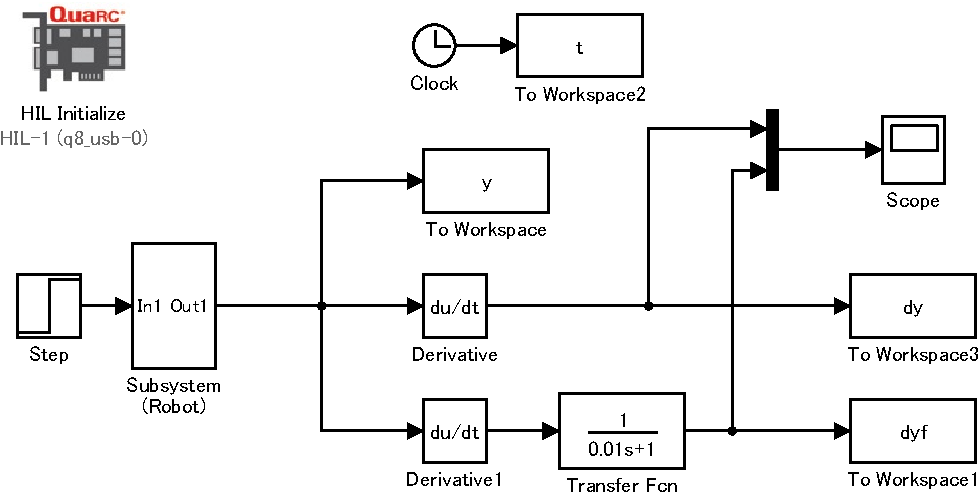
\includegraphics[scale=0.7]{sozai/ex_ident-crop.pdf}
  \caption{ex\_ident}
\end{figure}

\begin{figure}[h]
  \centering
  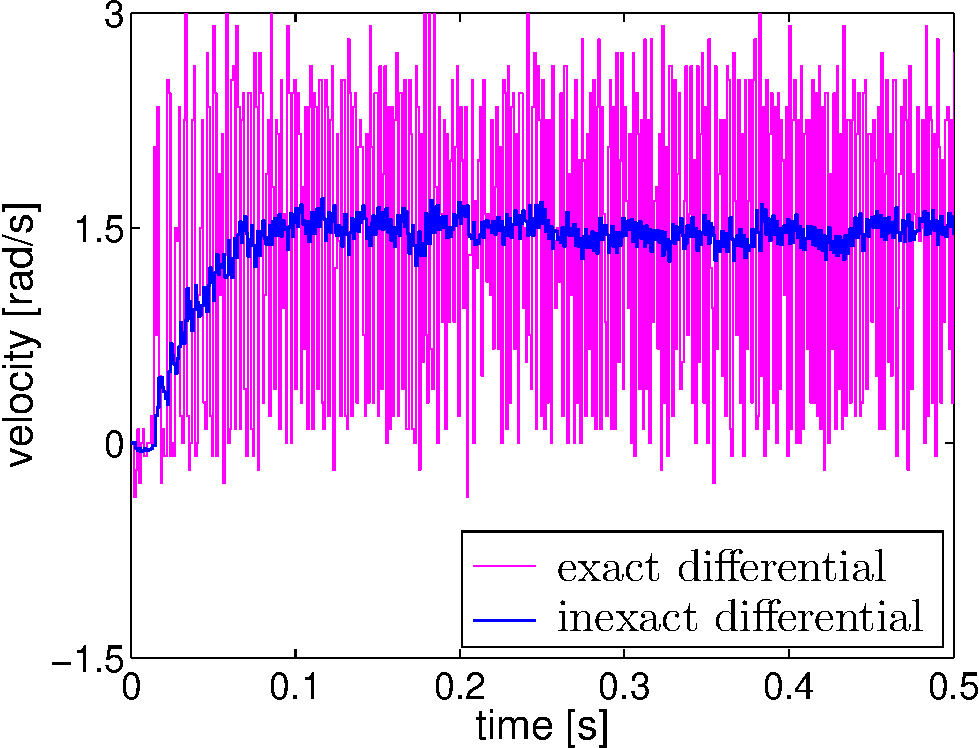
\includegraphics[scale=0.5]{sozai/figure_lowpass-crop.pdf}
  \caption{figure\_lowpass}
\end{figure}

\begin{figure}[h]
  \centering
  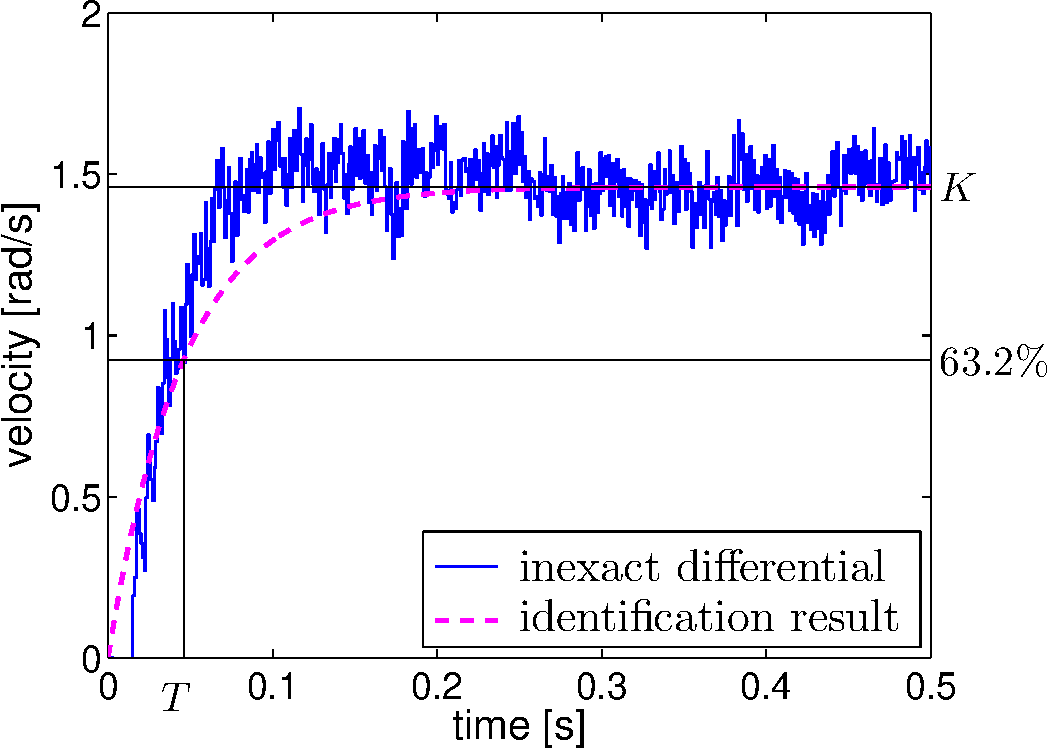
\includegraphics[scale=0.5]{sozai/figure_ident-crop.pdf}
  \caption{figure\_ident}
\end{figure}

\newpage

\subsubsection{実験考察}

実験により得られたパラメータは,表に示すように,ゲイン \( K = 1.46 \),
時定数 \( T = 0.046 \) ,および未知パラメータ \( a = 21.7 \),\( b = 31.8 \) である.
図5.2の結果より,ローパスフィルタを適用していない場合(exact differential)は,
観測雑音により信号に大きな振動が生じているのが確認できる.
一方,ローパスフィルタを適用した場合(inexact differential)では,
結果図5.3から得られたゲイン \( K = 1.46 \) は,
システムが入力ステップ応答に対して約63.2\%に達する値であり,
実験により同定された時定数 \( T = 0.046 \) は,
システムがこの値に収束するまでの応答時間を表している.
また, \( \frac{1}{\omega} = \frac{1}{100} \approx 0.01 \, 
\text{s} \) であるのに対し,同定されたシステムの時定数は \( T = 0.046 \, \text{s} \)
であることがわかる.

そして,カットオフ周波数は
\[
  f = \frac{\omega}{2 \pi} \approx 15.9 \, \text{[rad/s]}
\]
となる.
したがって,フィルタのカットオフ周波数はノイズ周波数 \( 100 \, \text{[rad/s]} \) よりも
低く設定されており,このフィルタによってノイズが効果的に減衰されると考えられる.
図5.2に示されるように,exact differential(フィルタ未適用)の場合には
高周波成分による大きな振動が観察されたが,
inexact differential(フィルタ適用)の場合にはノイズが減衰され,
信号が滑らかになっている.


\subsection{P-D 制御}

\begin{enumerate}
  \item (4.11) 式にしたがって P-D コントローラ (4.13) 式のパラメータを定め,表 5.2 を完成させよ.
        
  \item 図 5.2 の Simulink モデル "ex.pdcont.slx" を作成し,ディレクトリ D:\#student.5S\#group01\#pdcont に保存する.ただし,"Subsystem (P-D Controller)" の内部は各自作成する(角速度 $\dot{\theta}$ はローパスフィルタ $G_f(s) = \frac{1}{1 + 0.01s}$ に通す).
        
  \item 次に,表 5.2 に示す比例ゲイン $k_{\mathrm{P}}$,微分ゲイン $k_{\mathrm{D}}$ を,コマンドウィンドウで
        
        \(>> k_{\mathrm{P}} = ***; k_{\mathrm{D}} = ***;\)
        
        と入力(*** には表 5.2 の数字を入力する)した後,ビルドを行い,エラーがないことを確認する.
        また,"ex.pdcont.pdf" という名前の pdf ファイルを生成し,デスクトップ上の 
        "bcpdfcrop-multi.bat" により余白を取り除く.
        
  \item Scope と Scope1 を開き,リアルタイムで角度と操作量を観測できるようにする.レンズは付録 A.2 の図 A.6 に合わせる.
        
  \item センサ電圧が 0 [V] となる位置にアームを動かし,"ex.pdcont.slx" を実行する.実行ss終了後,コマンドウィンドウで
        
        
        >> save pdcont\_data1 t u y \(k_{\mathrm{P}} k_{\mathrm{D}}\)
        
        
        と入力し,データを
        
        \begin{itemize}
          \item "pdcont.data1.mat" ($\omega_M = 15, \zeta_M = 0.3$)
          \item "pdcont.data2.mat" ($\omega_M = 15, \zeta_M = 0.7$)
          \item "pdcont.data3.mat" ($\omega_M = 15, \zeta_M = 1$)
        \end{itemize}
        
        という名前の mat ファイルでディレクトリ D:\#student.5S\#group01\#pdcont に保存する.最後に,配布する M ファイル
        
        "autoplot\_pdcont.m"
        
        を実行することによって,MATLAB 上でグラフを作成する.グラフの pdf ファイルは自動的に生成される.
        
  \item 目標値を 0 に設定(Step の最終値を "0" に設定)し,また,終了時間を "inf" に設定する.$\omega_M$, $\zeta_M$ を表 5.2 のように与えた後,アームを平らに 45 [deg] 程度動かしてから手を放すとき,アームがどのように応答するか調べよ.
\end{enumerate}


\subsubsection{実験結果}
以下に結果を示す.

\begin{figure}[h]
  \centering
  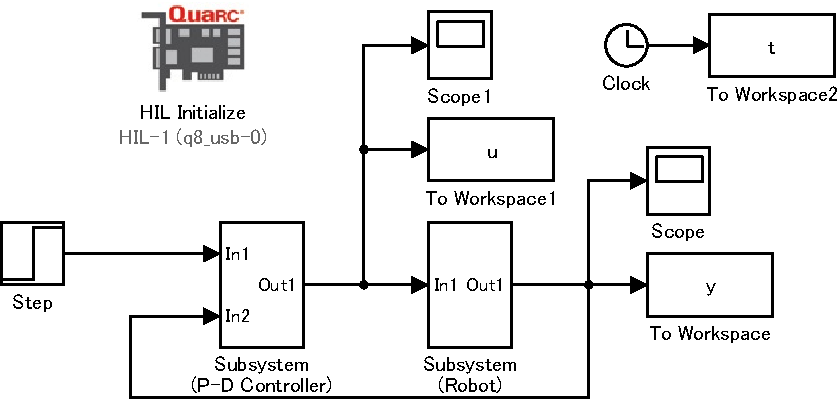
\includegraphics[scale=1]{sozai/ex_pdcont-crop.pdf}
  \caption{ex\_pdcont}
\end{figure}

\begin{table}[h]
  \centering
  \caption{P-D コントローラ}
  \begin{tabular}{|c|c|c|c|}
    \hline
    固有角周波数 $\omega_M$ & 減衰係数 $\zeta_M$ & 比例ゲイン $k_{\mathrm{P}}$ & 微分ゲイン $k_{\mathrm{D}}$ \\
    \hline
    15                      & 0.3                & 7.075                       & -0.399                      \\
    15                      & 0.7                & 7.075                       & -0.022                      \\
    15                      & 1                  & 7.075                       & 0.261                       \\
    \hline
  \end{tabular}
\end{table}

\begin{figure}[h]
  \centering
  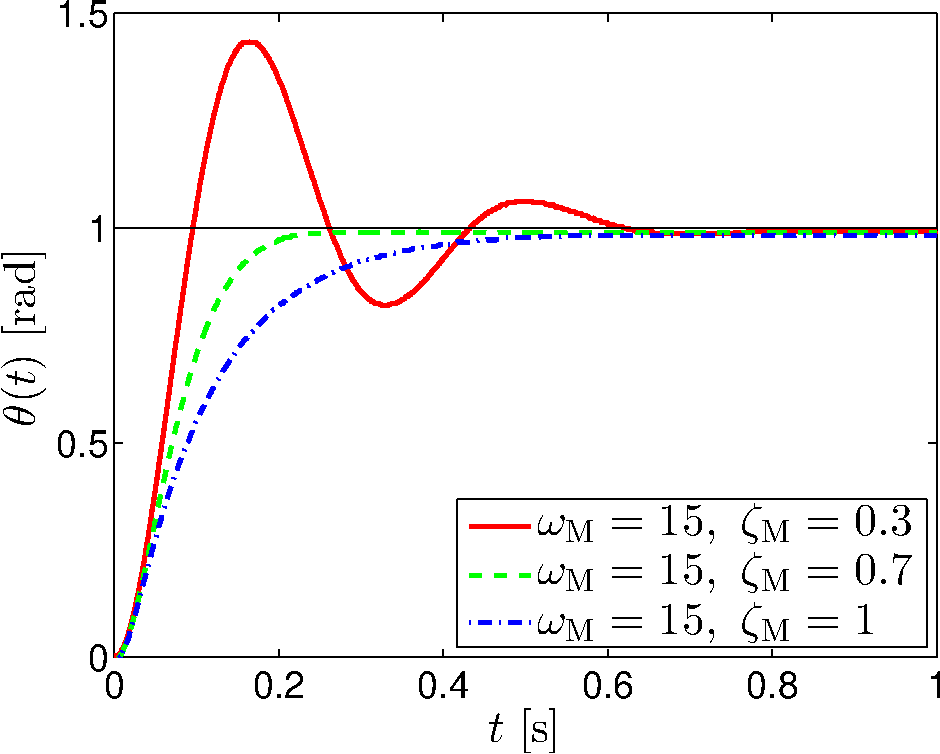
\includegraphics[scale=0.5]{sozai/figure_pdcont_angle-crop.pdf}
  \caption{ex\_pdcont}
\end{figure}

\begin{figure}[h]
  \centering
  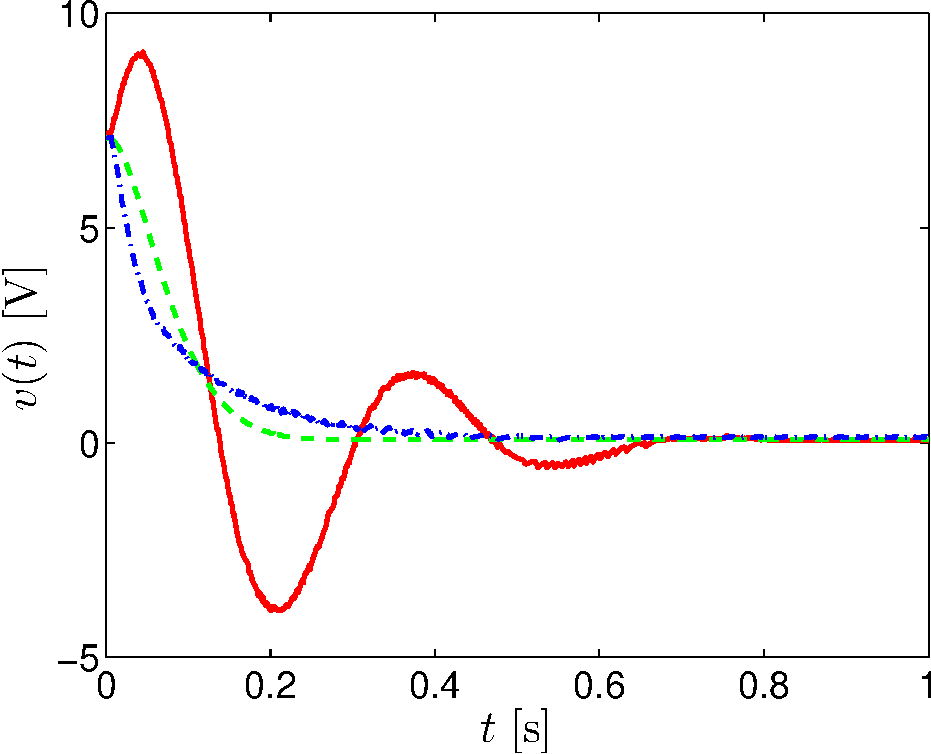
\includegraphics[scale=0.5]{sozai/figure_pdcont_volt-crop.pdf}
  \caption{ex\_pdcont}
\end{figure}

\newpage

(5) 減衰係数が大きくなるに連れ,即応性がなくなり,ゆっくりになりダンパの動きが見られた.

\subsubsection{実験考察}
微分動作は,制御対象の誤差の時間変化を考慮し,制御入力を調整するものである.
これにより応答の速度が向上し,オーバーシュートの抑制や立ち上がり時間の短縮が期待できる.
微分動作を加えることで,過渡応答が改善され,立ち上がり時の急激な変動が抑制されると考えられる.

次に,規範モデル式 (4.10) に基づくステップ応答と実験結果における定常偏差の違いについて述べる.
理論的な規範モデルは,理想的な条件での応答を示しているが,PD制御である場合,定常偏差が残る可能性がある.
このことは次の最終値の定理からも確認できる.
\[
  \lim_{t \to \infty} e(t) = \lim_{s \to 0} s E(s)
\]
積分動作がない場合,\( e(t) \) はゼロに収束せず,
定常偏差が残存することになる.
次に,減衰係数を変化させたときのアームの挙動について,
マスバネダンパ系の視点から考察する.マスバネダンパ系の運動方程式は以下のように表される.
\[
  m \ddot{z} + c \dot{z} + k z = f
\]
これを \( f \) について解くと,
\[
  f = m \ddot{z} + c \dot{z} + k z
\]
となる.ここで,\( m \) は質量,\( c \) はダンパ係数(減衰係数に関係),\( k \) はバネ定数
(固有角周波数に関係)である.
この系の伝達関数 \( P(s) \) は,出力を \( z(s) \) ,入力を \( f(s) \) として
\[
  P(s) = \frac{z(s)}{f(s)} = \frac{1}{m s^2 + c s + k}
\]
と表される.
さらに,この系を2次遅れ系の標準形に変換するため,分母の式を整理すると
\[
  P(s) = \frac{\frac{1}{m}}{s^2 + \frac{c}{m} s + \frac{k}{m}}
\]
となる.ここで,2次遅れ系の標準形
\[
  P(s) = \frac{\omega_n^2}{s^2 + 2 \zeta \omega_n s + \omega_n^2}
\]
と比較すると,固有角周波数 \( \omega_n \) と減衰係数 \( \zeta \) はそれぞれ以下のように表されることが
わかる.
\[
  \omega_n = \sqrt{\frac{k}{m}}, \quad \zeta = \frac{c}{2 \sqrt{m k}}
\]
これにより,バネ定数 \( k \) を変化させると固有角周波数 \( \omega_n \) が変化し,
ダンパ係数 \( c \) を変化させると減衰係数 \( \zeta \) が変化することがわかる.


\subsection{I-P制御}
\begin{enumerate}
  \item (4.18)式にしたがってI-Pコントローラ(4.14)式のパラメータを定め,表5.3を完成する.
  \item 図5.3のSimulinkモデル“ex\_ipcont.slx”を作成し,ディレクトリD:\#student\_5S\#group01\#ipcontに保存する.ただし,“Subsystem (I-P Controller)”の内容は各自で考える.
  \item 表5.3の比例ゲイン$k_{\mathrm{P}}$,積分ゲイン$k_{\mathrm{I}}$をコマンドウィンドウで
        \begin{verbatim}
  >> kP = ***; kI = ***;
  \end{verbatim}
        と入力し(***には表5.3の数値を入力する),ビルドを行い,エラーがないことを確認する.また,“ex\_ipcont.pdf”という名前のpdfファイルを生成し,デスクトップ上の“bcpdfcrop-multi.bat”により余白を取り除く.
        
  \item ScopeとScope1を開き,リアルタイムで角度と操作量を観測できるようにする.レンズは付録A.2の図A.7に合わせる.
        
  \item センサ電圧が0[V]となる位置にアームを動かし,“ex\_ipcont.slx”を実行する.実行終了後,コマンドウィンドウで
        \begin{verbatim}
  >> save ipcont_data1 t u y kP kI
  \end{verbatim}
        と入力し,データを
        \begin{itemize}
          \item “ipcont\_data1.mat” ($\omega_M = 15, \zeta_M = 0.3$)
          \item “ipcont\_data2.mat” ($\omega_M = 15, \zeta_M = 0.7$)
          \item “ipcont\_data3.mat” ($\omega_M = 15, \zeta_M = 1$)
        \end{itemize}
        という名前のmatファイルでディレクトリD:\#student\_5S\#group01\#ipcontに保存する.最後に,配布するMファイル
        \begin{verbatim}
  autoplot-ipcont.m
  \end{verbatim}
        を実行することによって,MATLAB上でグラフを作成する.グラフのpdfファイルは自動的に生成される.
        
\end{enumerate}

\subsubsection{実験結果}
\begin{figure}[h]
  \centering
  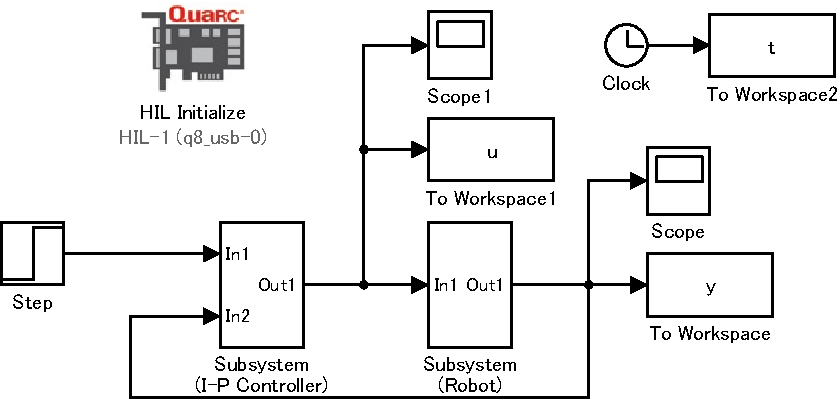
\includegraphics[scale=1]{sozai/ex_ipcont-crop.pdf}
  \caption{ex\_ipcont}
\end{figure}

\begin{table}[h]
  \centering
  \caption{I-Pコントローラ}
  \begin{tabular}{|c|c|c|c|}
    \hline
    固有角周波数$\omega_M$ & 減衰係数$\zeta_M$ & 比例ゲイン$k_{\mathrm{P}}$ & 積分ゲイン$k_{\mathrm{I}}$ \\
    \hline
    15                     & 0.3               & 6.14150                    & 153.53773                  \\
    15                     & 0.7               & 14.33018                   & 153.53773                  \\
    15                     & 1                 & 20.47169                   & 153.53773                  \\
    \hline
  \end{tabular}
\end{table}

\begin{figure}[h]
  \centering
  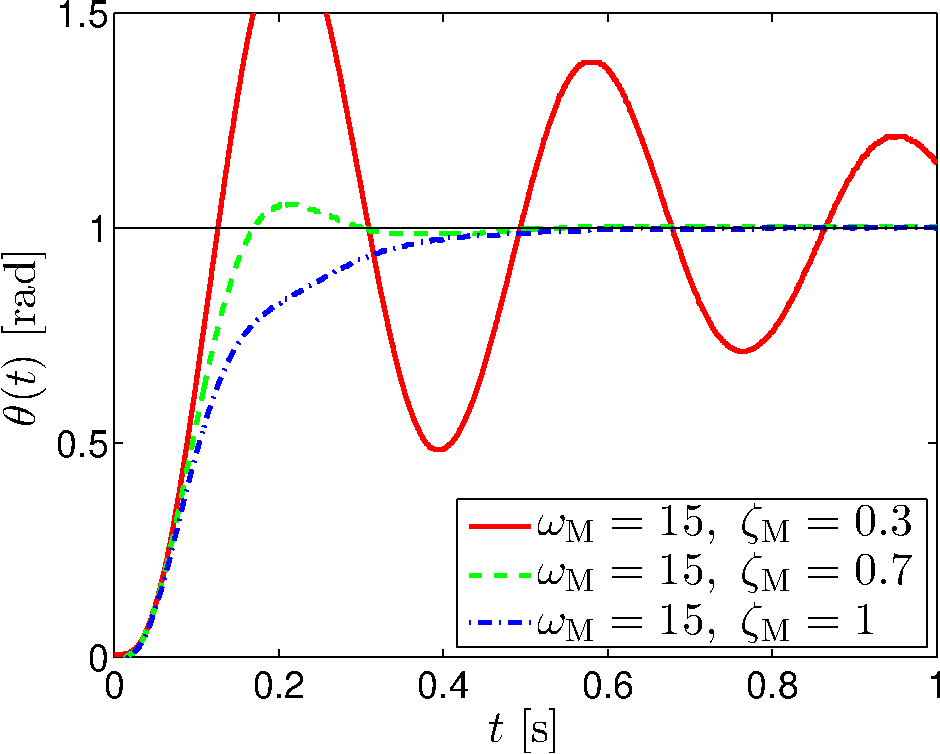
\includegraphics[scale=0.5]{sozai/figure_ipcont_angle-crop.pdf}
  \caption{ex\_ipcont}
\end{figure}

\begin{figure}[h]
  \centering
  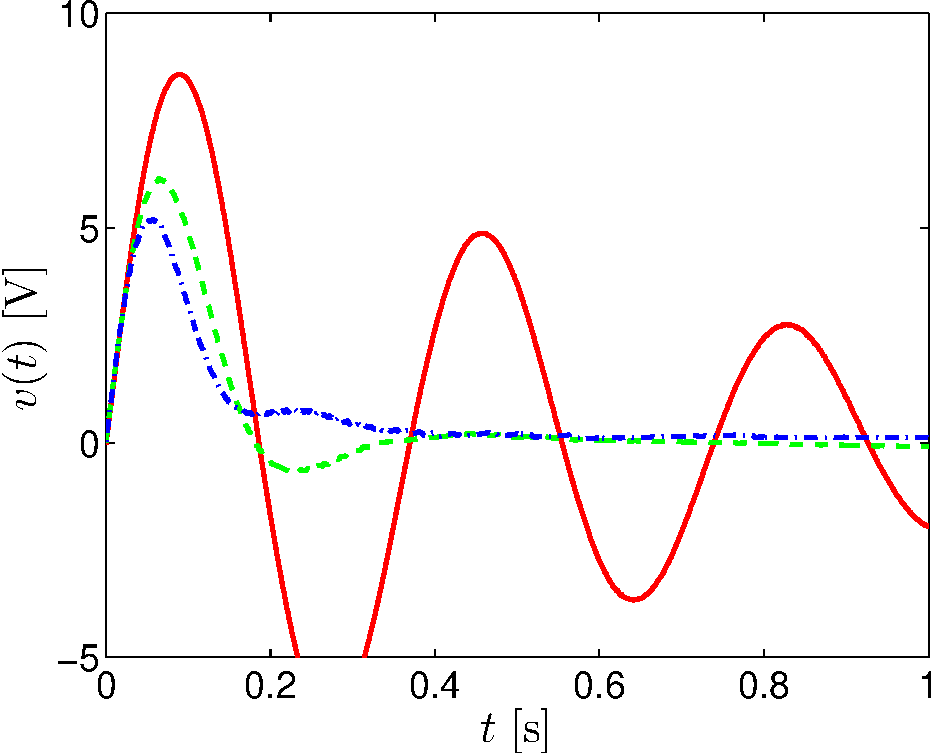
\includegraphics[scale=0.5]{sozai/figure_ipcont_volt-crop.pdf}
  \caption{ex\_ipcont}
\end{figure}

\newpage

\subsubsection{実験考察}
I-P制御は,偏差に積分動作を適用した量に基づいて,目標値の変化を滑らかにし,
その後に比例要素を作用させた操作量を出力します.
この制御構造により,I-P制御は目標値の急激な変化を緩和し,システムに与える影響を抑制する働きを持つ.
これは図5.9からも読み取れる.
P-D制御では積分動作がないため,外乱や負荷変動によって生じた定常偏差がそのまま残ってしまう一方,I-P制御
には積分動作が含まれているため,定常偏差が時間とともに収束し,最終的には目標値に到達する.
また,動作が規範モデルとことなる理由は,パラメータ調整に部分的モデルマッチング法が用いられているためである.
部分的モデルマッチング法は,特定の周波数帯域において理想モデルに近似するように設計されるが,
全体の応答を完全に再現するものではない.
したがって,高周波数成分や外乱の影響が含まれる実験結果においては,理想モデルと異なる結果が出たと考えられる.
また,PI制御には零点が含まれており,これによって特性が異なる.
具体的には,PI制御では零点の影響で応答が過渡的に速くなる傾向があるが,
I-P制御にはこの零点が存在しないため,応答はより滑らかで,
急激な変化が抑えられる.
この点で,I-P制御は目標値の変化に対して応答を穏やかにし,
システムが安定して追従するようになっている.


\subsection{I-PD制御}

\begin{enumerate}
  \item (4.22) 式にしたがって I-PD コントローラ (4.23) 式のパラメータを定め,表 5.4 を完成せよ.
        
  \item 次に,表 5.4 の比例ゲイン $k_{\mathrm{P}}$,積分ゲイン $k_{\mathrm{I}}$,微分ゲイン $k_{\mathrm{D}}$ を,コマンドウィンドウで次のように入力します.
        \begin{verbatim}
        kP = ***; kI = ***; kD = ***;
        \end{verbatim}
        
  \item Scope と Scope1 を開き,リアルタイムで角度と操作量を観測できるようにする.レジメは付録 A.2 の 図 A.8 に合わせる.
        
  \item センサ電圧が 0 [V] となる位置にアームを動かし,“ex\_ipdcont.slx” を実行する.実行終了後,コマンドウィンドウで
        \begin{verbatim}
  >> save ipdcont_data1 t u y kP kI kD
  \end{verbatim}
        と入力し,データを以下のファイルとして保存します.
        
        - “ipdcont\_data1.mat” ($\omega_M = 20, \alpha_{M1} = 2, \alpha_{M2} = 2$)
        - “ipdcont\_data2.mat” ($\omega_M = 20, \alpha_{M1} = 3, \alpha_{M2} = 3$)
        - “ipdcont\_data3.mat” ($\omega_M = 20, \alpha_{M1} = 2.15, \alpha_{M2} = 1.75$)
        
        これらの mat ファイルをディレクトリ D:\\\$student\_55\\group01\\ipdcont に保存します.最後に,以下の M ファイルを実行します.
        
        - “autoplot\_ipdcont.m”
        
        この実行によって,MATLAB 上でグラフを作成し,グラフの pdf ファイルは自動的に生成されます.
\end{enumerate}

\subsubsection{実験結果}
\begin{figure}[h]
  \centering
  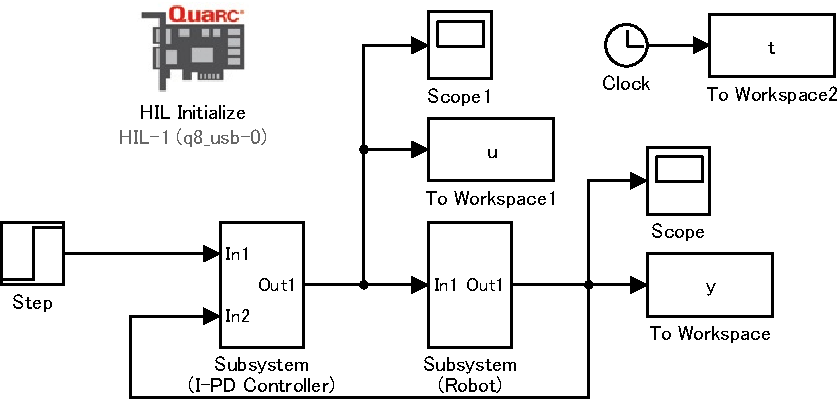
\includegraphics[scale=1]{sozai/ex_ipdcont-crop.pdf}
  \caption{ex\_ipdcont}
\end{figure}

\begin{table}[H]
  \centering
  \caption{I-PD コントローラ}
  \begin{tabular}{|c|c|c|c|c|c|}
    \hline
    $\omega_M$ & $\alpha_{M1}$ & $\alpha_{M2}$ & 比例ゲイン $k_{\mathrm{P}}$ & 積分ゲイン $k_{\mathrm{I}}$ & 微分ゲイン $k_{\mathrm{D}}$ \\ \hline
    20         & 2             & 2             & 25.157                      & 251.572                     & 0.575                       \\ \hline
    20         & 3             & 3             & 37.736                      & 251.572                     & 1.204                       \\ \hline
    20         & 2.15          & 1.75          & 27.044                      & 251.572                     & 0.418                       \\ \hline
  \end{tabular}
\end{table}


\begin{figure}[h]
  \centering
  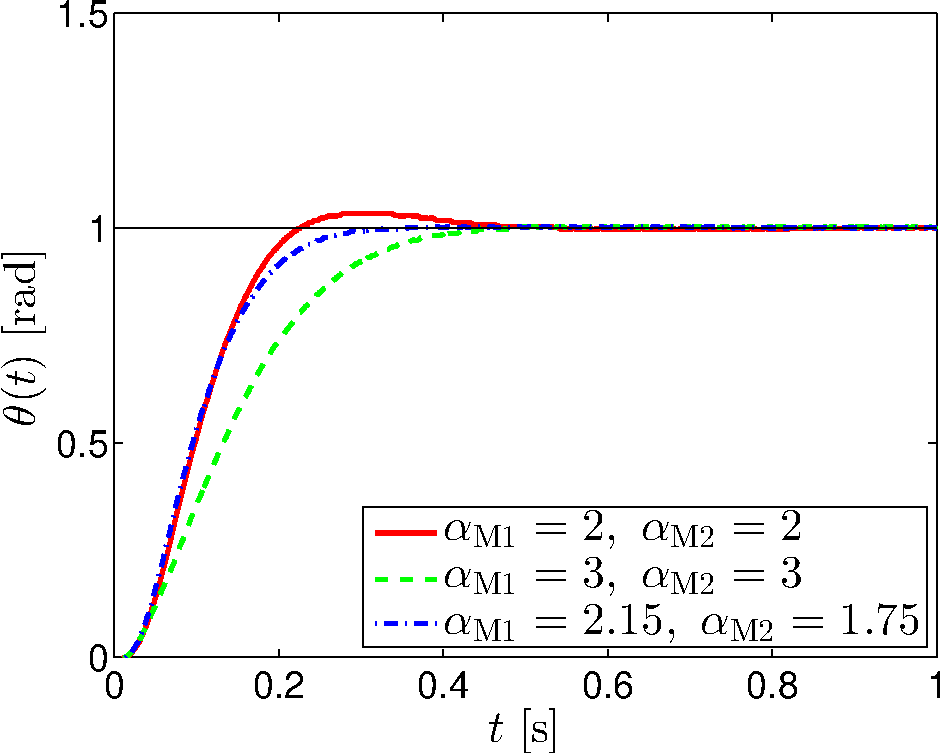
\includegraphics[scale=0.5]{sozai/figure_ipdcont_angle-crop.pdf}
  \caption{figure\_ipdcont\_angle}
\end{figure}

\begin{figure}[h]
  \centering
  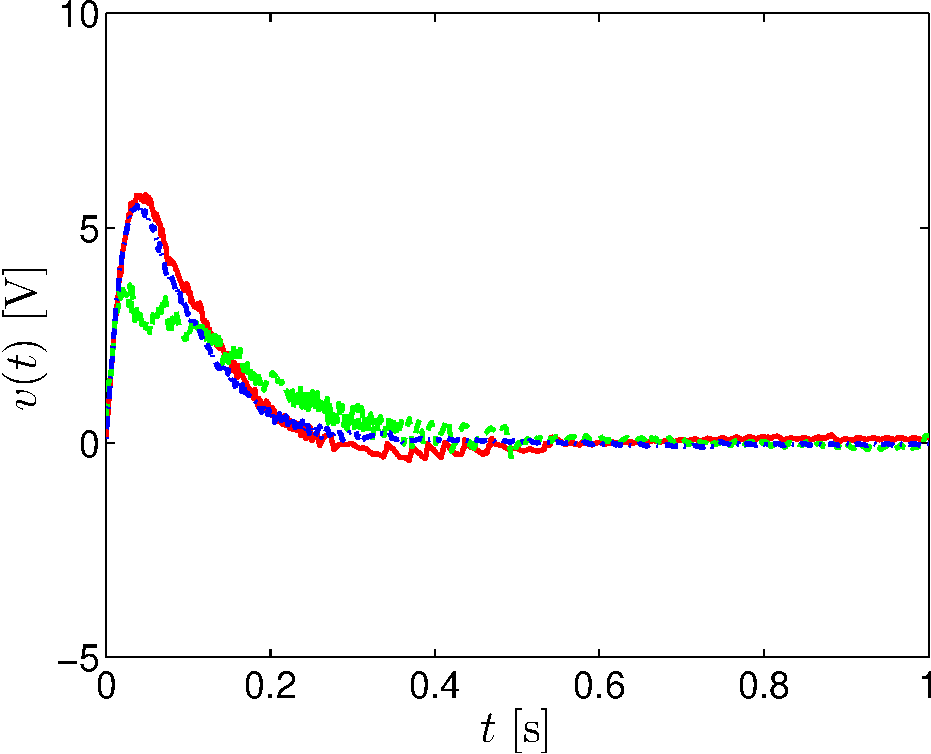
\includegraphics[scale=0.5]{sozai/figure_ipdcont_volt-crop.pdf}
  \caption{figure\_ipdcont\_volt}
\end{figure}

\newpage

\subsubsection{実験考察}
I-PD制御は,比例項(\( k_{\mathrm{P}} \))と積分項(\( k_{\mathrm{I}} \)),
および微分項(\( k_{\mathrm{D}} \))が組み合わさることで,
応答速度と定常精度が良くなっている.
図5.12より,角度応答では目標値への到達が速く,
また定常状態での偏差がほとんどないことがわかる.
これは積分項によって定常偏差が補正されるため,P-D制御と比較して定常偏差がほぼなくなっているためだと考えられる.
また,I-P制御と比較しても過渡応答が速く,振動が抑えられている.

一方で,図5.13に示される電圧応答においては,微分ゲインが大きいときに振動が見られる.
これは微分項が高周波成分やノイズに敏感であるためであり,
急激な変動に対して過大な操作量が発生しやすいためである.
そのため,一般的に微分動作の前にローパスフィルターなどのフィルターを通すことが一般的である.


\section{調査課題}

\subsection*{1}
ポテンショメータは,可変抵抗器の一種であり,
主に位置や角度を測定するためのセンサとして使用される.
その動作原理は,接点(スライダー)を抵抗体上で移動させることによって,
抵抗値を変化させ,その変化によって位置や角度を検出する.
抵抗体の両端に電圧を印加し,スライダーの位置に応じた電圧が出力されるため,位置情報が得られる.
\[
  \text{出力電圧} = \frac{\text{スライダーの位置}}{\text{全抵抗体の長さ}} \times \text{印加電圧}
\]
また,ポテンショメータはアブソリュート位置センサであるため,
電源のオン・オフに関係なく位置情報を保持できる.
しかし,スライダーと抵抗体の接触部分が摩耗しやすいため,
耐久性や寿命が求められる用途には不向きである.

\subsection*{2}
A/D変換は,アナログ信号をデジタル信号に変換するプロセスである.
アナログ信号が時間的および値の上で連続的であるのに対し,
デジタル信号は離散的なサンプル点と有限のビットで表現される.
まず,サンプリングにより,アナログ信号の時間的に連続したデータを一定の時間間隔で分割して離散化する.
次に,量子化を行う.
量子化は,サンプリングによって得られた信号の値を有限のビット数で表現できるように離散化するプロセスである.
量子化の精度はビット数に依存し,ビット数が多いほどより詳細なアナログ信号の情報を保持できる.
最後に,符号化が行われ,量子化された値をデジタル形式として記録する.
D/A変換は,デジタル信号を再びアナログ信号に戻すプロセスである.
デジタル信号は不連続なデータで構成されているため,
変換によって生成されるアナログ信号は理想的な連続信号とは異なる場合があるが,
近似的な再現が可能である.


\subsection*{3}
レンジが \(\pm 5\) V,分解能が12ビットの場合,アナログ出力の電圧は,
\[
  \text{1 LSB} = \frac{10 \, \text{V}}{4096} = \frac{10}{4096} \approx 0.00244 \, \text{V}
\]
次に,0x0C00のデジタル値をアナログ値に変換する.0x0C00は10進数に直すと3072であるため,

\[
  \text{アナログ値} = (3072) \times 0.00244 \, \text{V} - 5 \, \text{V} = 2.5 \, \text{V}
\]

よって0x0C00をD/A変換するとアナログ値は2.5[V]となる

\subsection*{4}
式 \(4.9\) は以下の通りである.
\[
  T(s) = \frac{\omega_n^2}{s^2 + 2 \zeta \omega_n s + \omega_n^2}, \quad \omega_n = \sqrt{b k_{\mathrm{P}}}, \quad \zeta = \frac{a + b k_{\mathrm{D}}}{2 \omega_n}
\]
システムの運動方程式に比例微分(PD)制御を適用すると,次の式が得られる.
\[
  m \frac{d^2 x}{dt^2} + c \frac{dx}{dt} + kx = k_{\mathrm{P}} e + k_{\mathrm{D}} \frac{de}{dt}
\]
ここで,簡略化のために \( b = \frac{1}{m} \) および \( a = \frac{c}{m} \) とおくと,上記の式は次のように表される.
\[
  \frac{d^2 x}{dt^2} + a \frac{dx}{dt} + bx = b k_{\mathrm{P}} e + b k_{\mathrm{D}} \frac{de}{dt}
\]

ラプラス変換を適用して,ラプラス変数 \( s \) を用いて表現する.これにより次の式が得られる.
\[
  (s^2 + as + b) X(s) = b k_{\mathrm{P}} E(s) + b k_{\mathrm{D}} s E(s)
\]
ここで,出力と入力の比 \( T(s) = \frac{X(s)}{E(s)} \) を整理すると,以下の伝達関数が得られる.
\[
  T(s) = \frac{X(s)}{E(s)} = \frac{b k_{\mathrm{P}} + b k_{\mathrm{D}} s}{s^2 + as + b}
\]

ここで,自然周波数 \( \omega_n \) と減衰係数 \( \zeta \) を次のように定義する.
\[
  \omega_n = \sqrt{b k_{\mathrm{P}}}
\]
\[
  \zeta = \frac{a + b k_{\mathrm{D}}}{2 \omega_n}
\]

これらを代入し,伝達関数を整理すると次の式が得られる.
\[
  T(s) = \frac{\omega_n^2}{s^2 + 2 \zeta \omega_n s + \omega_n^2}
\]


式 \(4.20\) は次のように与えられる.
\[
  T(s) = \frac{b k_{\mathrm{I}}}{s^3 + (a + b k_{\mathrm{D}})s^2 + b k_{\mathrm{P}} s + b k_{\mathrm{I}}}
\]
PID制御を適用したシステムの運動方程式は,次のように与えられる.
\[
  m \frac{d^2 x}{dt^2} + c \frac{dx}{dt} + kx = k_{\mathrm{P}} e + k_{\mathrm{D}} \frac{de}{dt} + k_{\mathrm{I}} \int e \, dt
\]
ここで,簡略化のために \( b = \frac{1}{m} \) および \( a = \frac{c}{m} \) とおくと,上記の式は次のように書き直される.
\[
  \frac{d^2 x}{dt^2} + a \frac{dx}{dt} + bx = b k_{\mathrm{P}} e + b k_{\mathrm{D}} \frac{de}{dt} + b k_{\mathrm{I}} \int e \, dt
\]

ラプラス変換を適用して,ラプラス変数 \( s \) を用いて表現すると,積分項 \( \int e \, dt \) のラプラス変換は \( \frac{E(s)}{s} \) となり,以下の式が得られる.
\[
  (s^2 + as + b) X(s) = b k_{\mathrm{P}} E(s) + b k_{\mathrm{D}} s E(s) + \frac{b k_{\mathrm{I}}}{s} E(s)
\]

次に,この式を \( X(s) \) と \( E(s) \) の関係として整理する.右辺を \( E(s) \) でくくり出すと,以下のようになる.
\[
  (s^2 + as + b) X(s) = \left( b k_{\mathrm{P}} + b k_{\mathrm{D}} s + \frac{b k_{\mathrm{I}}}{s} \right) E(s)
\]

ここで,\( T(s) = \frac{X(s)}{E(s)} \) として,両辺を \( E(s) \) で割ると次のようになる.
\[
  T(s) = \frac{X(s)}{E(s)} = \frac{b k_{\mathrm{I}}}{s^3 + (a + b k_{\mathrm{D}}) s^2 + b k_{\mathrm{P}} s + b k_{\mathrm{I}}}
\] \newpage

\newpage

%%%%%%%%%%%%%%%%%%%%%%%%%%%%%%%%%%%%%%%%%%%%%%%%%%%%%%%%%%%%%%%%%%%%%%%%%%%%%
%%%%%% 参考文献 %%%%%%%%%%%%%%%%%%%%%%%%%%%%%%%%%%%%%%%%%%%%%%%%%%%%%%%%%%%
%%%%%%%%%%%%%%%%%%%%%%%%%%%%%%%%%%%%%%%%%%%%%%%%%%%%%%%%%%%%%%%%%%%%%%%%%%%%%
% !TEX root = main.tex
\newpage
%%%%%%%%%%%%%%%%%%%%%%%%%%%%%%%%%%%%%%%%%%%%%%%%%%%%%%%%%%%%%%%%%%%%%%%%
\begin{center}
	\section*{参\,考\,文\,献}                      %% ここに番号をつけない
\end{center}
\addcontentsline{toc}{section}{参考文献} %% 目次に番号をつけない
%%%%%%%%%%%%%%%%%%%%%%%%%%%%%%%%%%%%%%%%%%%%%%%%%%%%%%%%%%%%%%%%%%%%%%%%

\begin{thebibliography}{9}
	\bibitem{ref1} 細田耕:実践ロボット制御,オーム社,2019.
	\bibitem{ref2} 株式会社アールティ:3自由度ロボットの順運動学と逆運動学,<https://rt-net.jp/humanoid/archives/2652>(2024年4月1日閲覧).
	\bibitem{ref3} 酒井幸市:デジタル画像処理入門,コロナ社,2001.
	\bibitem{ref4} 北山直洋:Pythonで始めるOpenCV 4プログラミング,株式会社カットシステム,2019.
\end{thebibliography}


% ******************************************* \newpage

%%%%%%%%%%%%%%%%%%%%%%%%%%%%%%%%%%%%%%%%%%%%%%%%%%%%%%%%%%%%%%%%%%%%%%%%%%%%%
%%%%%% 付録 %%%%%%%%%%%%%%%%%%%%%%%%%%%%%%%%%%%%%%%%%%%%%%%%%%%%%%%%%%%%%%%
%%%%%%%%%%%%%%%%%%%%%%%%%%%%%%%%%%%%%%%%%%%%%%%%%%%%%%%%%%%%%%%%%%%%%%%%%%%%%
%\makeatletter
     \renewcommand{\theequation}{%
          A.\arabic{equation}}
     \@addtoreset{equation}{section}
\makeatother

\makeatletter
     \renewcommand{\thetable}{%
          A.\arabic{table}}
     \@addtoreset{table}{section}
\makeatother

\makeatletter
     \renewcommand{\thefigure}{%
          A.\arabic{figure}}
     \@addtoreset{figure}{section}
\makeatother

\makeatletter
     \renewcommand{\thesubsection}{%
          A.\arabic{subsection}}
     \@addtoreset{subsection}{section}
\makeatother

\makeatletter
     \renewcommand{\thesubsubsection}{%
          A.\arabic{subsection}.\arabic{subsubsection}}
     \@addtoreset{subsubsection}{section}
\makeatother
 \newpage

\end{document}
